%% 전농사거리 소음현황조사 결과보고서(제출본)
%% 컴파일: xelatex (목차·전체 쪽수 반영을 위해 2회)
%% 본 문서는 생성형 AI(Claude)를 활용하여 작성되었음.
\documentclass[10.5pt,a4paper]{article}
\usepackage[a4paper,top=22mm,bottom=24mm,left=22mm,right=22mm,headsep=6mm,footskip=10mm]{geometry}
\usepackage{fontspec}
\usepackage{xetexko}
\IfFontExistsTF{Noto Serif CJK KR}{%
  \setmainfont{Noto Serif CJK KR}\setsansfont{Noto Sans CJK KR}%
  \setmainhangulfont{Noto Serif CJK KR}\setsanshangulfont{Noto Sans CJK KR}%
  \setmonohangulfont{Noto Sans CJK KR}[Scale=0.85]}{%
  \setmainfont{Times New Roman}\setsansfont{Apple SD Gothic Neo}%
  \setmainhangulfont{AppleMyungjo}[AutoFakeBold=2.5]\setsanshangulfont{Apple SD Gothic Neo}%
  \setmonohangulfont{Apple SD Gothic Neo}[Scale=0.85]}
\IfFontExistsTF{DejaVu Sans Mono}{\setmonofont{DejaVu Sans Mono}[Scale=0.82]}{%
  \setmonofont{DejaVuSansMono.ttf}[Scale=0.82,BoldFont=DejaVuSansMono-Bold.ttf]}

\usepackage{amsmath,amssymb}
\usepackage{array,booktabs,longtable,tabularx,makecell}
\usepackage[table]{xcolor}
\usepackage{graphicx}\usepackage{float}
\usepackage{enumitem}
\usepackage{needspace}
\usepackage{titlesec}
\usepackage{fancyhdr}
\usepackage{lastpage}
\usepackage[font=small,labelsep=colon,skip=4pt]{caption}
\usepackage[hidelinks]{hyperref}
\linespread{1.3}
\setlength{\parindent}{0pt}
\setlength{\parskip}{0.45em}
\setlength{\tabcolsep}{4pt}
\renewcommand{\arraystretch}{1.25}
\setlist{itemsep=0.15em,topsep=0.3em,leftmargin=1.6em}
\captionsetup[table]{name=표}
\captionsetup[figure]{name=그림}
\setcounter{secnumdepth}{3}
\setcounter{tocdepth}{2}
\definecolor{navy}{HTML}{1F3864}
\definecolor{headfill}{HTML}{D9E2F3}
\definecolor{inp}{HTML}{FFF8DC}
\definecolor{lab}{HTML}{F2F2F2}
\definecolor{team1}{HTML}{DDEBF7}
\definecolor{team2}{HTML}{E2EFDA}
\renewcommand{\thesection}{\arabic{section}.}
\renewcommand{\thesubsection}{\arabic{section}.\arabic{subsection}}
\renewcommand{\thesubsubsection}{\thesubsection.\arabic{subsubsection}}
\titleformat{\section}{\sffamily\Large\bfseries\color{navy}}{\thesection}{0.6em}{}
\titleformat{\subsection}{\sffamily\large\bfseries\color{navy}}{\thesubsection}{0.6em}{}
\titleformat{\subsubsection}{\sffamily\normalsize\bfseries}{\thesubsubsection}{0.6em}{}
\titlespacing*{\section}{0pt}{1.1em}{0.5em}
\titlespacing*{\subsection}{0pt}{0.9em}{0.4em}
\newcommand{\Laeq}{\ensuremath{L_{\mathrm{Aeq}}}}
\newcommand{\TBD}{\textcolor{gray}{[측정 후 기입]}}
\newcommand{\IN}{[\quad]}
\newcommand{\hd}[1]{\cellcolor{headfill}\textbf{\sffamily #1}}
\newcommand{\ip}{\cellcolor{inp}}
\newcommand{\lb}{\cellcolor{lab}}
\newcommand{\hr}[1]{\rule[-0.35\dimexpr#1\relax]{0pt}{#1}}
\newcommand{\notebox}[2][lab]{\par\noindent\colorbox{#1}{\parbox{\dimexpr\linewidth-2\fboxsep}{\small #2}}\par}
\renewcommand{\contentsname}{목차}
\pagestyle{fancy}\fancyhf{}
\fancyhead[L]{\small\sffamily 결과보고서}
\fancyhead[R]{\small\sffamily 전농사거리 소음현황조사}
\fancyfoot[L]{\scriptsize\sffamily\color{gray} 본 문서는 생성형 AI(Claude)를 활용하여 작성되었음}
\fancyfoot[R]{\small\sffamily \thepage\ / \pageref*{LastPage}}
\renewcommand{\headrulewidth}{0.4pt}
\fancypagestyle{plain}{\fancyhf{}\fancyfoot[L]{\scriptsize\sffamily\color{gray} 본 문서는 생성형 AI(Claude)를 활용하여 작성되었음}%
  \fancyfoot[R]{\small\sffamily \thepage\ / \pageref*{LastPage}}\renewcommand{\headrulewidth}{0pt}}
\newcolumntype{L}[1]{>{\raggedright\arraybackslash}p{\dimexpr #1\linewidth-2\tabcolsep\relax}}
\newcolumntype{C}[1]{>{\centering\arraybackslash}p{\dimexpr #1\linewidth-2\tabcolsep\relax}}
\newcommand{\mn}{\ensuremath{-}}
\newcommand{\NA}{\textcolor{gray}{미측정}}
\graphicspath{{../../field_measurement/2026-10-22/figures/}}
\begin{document}
\begin{titlepage}
\centering\vspace*{40mm}
{\sffamily\Huge\bfseries\color{navy} 전농사거리 소음현황조사 결과보고서\par}
\vspace{6mm}
{\sffamily\large 현재 소음도 평가와 소음지도 시뮬레이션 검증\par}
\vspace{18mm}
{\renewcommand{\arraystretch}{1.5}
\begin{tabular}{>{\raggedright\arraybackslash}p{38mm}>{\raggedright\arraybackslash}p{90mm}}
\toprule
\cellcolor{headfill}\textbf{\sffamily 과목} & 소음진동설계 \\ \midrule
\cellcolor{headfill}\textbf{\sffamily 대상} & 전농사거리 동쪽 접근로(사가정로) 도로변 \\ \midrule
\cellcolor{headfill}\textbf{\sffamily 측정일} & 2026년 10월 22일(목) 16:15--16:51 \\ \midrule
\cellcolor{headfill}\textbf{\sffamily 작성일} & 2026년 10월 28일 \\ \midrule
\cellcolor{headfill}\textbf{\sffamily 작성자} & 전현수 \\ \midrule
\cellcolor{headfill}\textbf{\sffamily 문서 상태} & 제출본(검토 의견 반영, 2026-10-28) \\ \midrule
\cellcolor{headfill}\textbf{\sffamily 적용 기준} & 2026-10-19·21 확인본 기준(제출 시점 재확인 안 함) \\
\bottomrule
\end{tabular}}
\vfill
\notebox{\textbf{본 문서는 생성형 AI(Claude)를 활용하여 작성되었음.} 측정값과 계산값은 저장소의 분석 결과(field\_measurement/2026-10-22, 02\_분석보고서.md 및 results/*.csv)를 옮긴 것이다. 기준값·조항은 측정계획서에서 국가법령정보센터 원문으로 확인한 값을 썼다. 확인하지 못한 항목은 `미확인', 측정하지 않은 항목은 `미측정'으로 표시했다.}
\end{titlepage}
\tableofcontents
\clearpage

%% ------------------------------------------------------------------
\section{요약}
\small
\begin{longtable}{L{0.24}L{0.76}}
\toprule
\hd{항목} & \hd{내용} \\ \midrule
\endhead
\bottomrule
\endlastfoot
측정 일시·지점 수 & 2026-10-22(목) 16:15--16:51. 사가정로 양쪽 도로변 2지점(지점1 북측 사가정로 123 앞, 지점2 남측 사가정로 148 앞)에서 10분씩 3회 동시 측정했다. 교통량도 같은 시간에 계수했다. \\ \midrule
기준 비교 결과(참고 평가, 목적 가) & 낮 측정소음도(산술평균, 정수)는 두 지점 모두 69 dB(A)다(용도지역은 토지이음으로 확인). 지점2(제3종일반주거지역, 도로변 ``나'')는 환경기준 65를 4 dB 넘고, 지점1(근린상업지역, 도로변 ``다'')은 기준 70 이하다. 도로 관리기준은 주간 69 dB(A)로, 주거지역 쪽 가목(68)은 1 dB 넘고 상업지역 쪽 나목(73)은 기준 이하다. 다만 측정 횟수와 회차 간격 요건을 채우지 못했다(낮 3회, 13분 간격). 따라서 이 값은 \textbf{참고 평가}다. 밤 시간대는 측정하지 않아 \textbf{평가 불가}다. \\ \midrule
시뮬레이션 비교 결과(목적 나) & 측정 교통량과 규정 속도 50 km/h를 넣은 모델(RLS-19 + ISO 9613-2)은 측정값보다 높게 계산했다. 차이는 측정 $-$ 계산 평균 $-$8.3 dB, 표준편차 0.65 dB($n=6$)다. 고시 기준(평균 $\pm$3 dB)을 넘는다. 속도를 30 km/h로 낮춰도 $-$5.7 dB가 남는다. 지점 간 차이(지점2 $-$ 지점1)는 측정 +0.5 dB, 모델 +0.7 dB로 비슷하다. \\ \midrule
소음지도(참고) & 같은 교통량으로 주간 소음지도를 사가정로 50·30 km/h로 그렸다(6.8절). 68 dB(A)를 넘는 벽면·층은 50 km/h에서 9.9 \%(200동), 30 km/h에서 7.5 \%(188동)다. 30 km/h로 낮추면 사가정로 변만 2.6--2.9 dB 줄고, 격자의 초과 비율은 34.4 \%에서 33.0 \%로 1.4 \%p 준다. 이 조건은 측정보다 5--8 dB 높게 계산되므로 초과 범위는 과대 추정일 수 있다. \\ \midrule
주요 한계 & 평일 오후 한 시간대에서만 10분씩 3회 측정했다. 다음 항목은 측정하지 않았다: 주행속도, 이륜차 별도 계수, 노면 종류, 현장 기상(기상은 약 8 km 떨어진 기상청 서울 관측소 값으로 대신함). 지점1 교정 수치는 기록되지 않았다. 측정 지점은 사가정로 한 도로뿐이다. \\ \midrule
소음지도 작업에 대한 시사점 & 이 구간에서는 모델의 절대 레벨이 측정보다 5--8 dB 높다. 차이의 대부분은 입력 가정에 따라 달라진다: 노면, 속도, 차종 분류. 따라서 소음지도 결과를 쓰기 전에 다음 세 가지를 실측하고 다시 검증해야 한다: 주행속도, 3.5 t 기준 화물차와 이륜차 분리 계수, 노면 종류. \\*
\end{longtable}
\addtocounter{table}{-1}
\normalsize

%% ------------------------------------------------------------------
\section{조사 개요}
\subsection{목적}
\begin{itemize}
\item 가. 현재 소음도 조사: 전농사거리 주변의 소음피해 현황을 국내 기준과 비교·평가
\item 나. 시뮬레이션 검증: 측정값을 소음지도 소프트웨어(RLS-19 + ISO 9613-2) 계산값과 같은 위치·조건에서 비교
\end{itemize}

\subsection{일시·인원·장비}
\small
\begin{longtable}{L{0.26}L{0.74}}
\toprule
\hd{항목} & \hd{내용} \\ \midrule
\endhead
\bottomrule
\endlastfoot
측정일·요일 & 2026-10-22(목), 평일 \\ \midrule
예비일 사용 여부·이유 & 사용하지 않음 \\ \midrule
회차별 시각 & 1회 16:15--16:25, 2회 16:28--16:38, 3회 16:41--16:51(각 10분, 두 지점 동시). 두 소음계의 시작 시각은 2--3 s 차이 난다 \\ \midrule
조사 인원·역할(2팀) & 총 5명: 김도협, 송기명, 임양록, 임영택, 전현수(가나다순). 2개 조로 나뉘어 지점1과 지점2에서 동시에 측정했다. 원자료 폴더 이름으로 보면 지점1 소음계는 임양록, 지점2 소음계는 임영택이 맡았다. 그 밖의 조 배정과 역할은 기록되지 않았다 \\ \midrule
측정점 & 지점1: 사가정로 123 앞, 도로 북측 보도. 건물 벽에서 1.001 m, 도로끝선까지 4.213 m, 마이크 높이 1.309 m. 지점2: 전농동SK아파트 상가 입구(사가정로 148) 앞, 도로 남측 보도. 건물 벽에서 1.13 m(야장 판독), 도로끝선까지 3.321 m, 마이크 높이 1.312 m. 전농사거리 중심에서 지점1은 약 88 m, 지점2는 약 100 m 떨어져 있다 \\
\end{longtable}
\addtocounter{table}{-1}
\normalsize
\small
\begin{longtable}{C{0.13}C{0.15}C{0.20}C{0.14}C{0.10}C{0.28}}
\toprule
\hd{장비 ID} & \hd{조·측정점} & \hd{모델} & \hd{일련번호} & \hd{등급} & \hd{교정기(표시값)} \\ \midrule
\endhead
\bottomrule
\endlastfoot
SLM-1 & 1조 · 지점1 & RION NL-62 (1/3옥타브 NX-62RT) & 511765 & 클래스 1 & 94 dB, 1 kHz. 교정 수치 미기록 \\ \midrule
SLM-2 & 2조 · 지점2 & RION NL-62 (1/3옥타브 NX-62RT) & 511778 & 클래스 1 & 94 dB, 1 kHz. 측정 전 93.7, 측정 후 94.0 dB \\
\end{longtable}
\addtocounter{table}{-1}
\normalsize
{\small 두 소음계 모두 방풍망을 달았다(WS-10 보정 설정, 사용자 확인). 교정기 모델명은 기록되지 않았다.\par}

\subsection{적용 기준}
\footnotesize
\begin{longtable}{L{0.16}L{0.46}L{0.38}}
\toprule
\hd{구분} & \hd{문서} & \hd{현행본(2026-10-19·21 확인)} \\ \midrule
\endhead
\bottomrule
\endlastfoot
측정방법 & 소음·진동공정시험기준 ES 03301.1c, ES 03304.1d, ES 03300.c & 국립환경과학원고시 제2026-39호(2026-09-14) \\ \midrule
환경기준 & 환경정책기본법 시행령 [별표 1] 2. 소음 & 대통령령 제36726호(2026-10-08 시행) \\ \midrule
관리기준 & 소음·진동관리법 시행규칙 [별표 11] 1. 도로 & 기후에너지환경부령 제42호(2026-06-22 시행) \\ \midrule
측정점 선정·검증 & 소음지도의 작성방법 별표 2(제12호 다목, 제14호 라목, 제15호) & 기후에너지환경부고시 제2026-19호(2026-01-18 시행) \\ \midrule
도로 소음 계산 & RLS-19(Richtlinien für den Lärmschutz an Straßen, 2019) + ISO 9613-2 & 소음지도 소프트웨어 구현 \\
\end{longtable}
\addtocounter{table}{-1}
\normalsize
{\small 개정 여부 재확인: 측정계획서 작성 시(2026-10-19·21) 확인한 현행본을 그대로 썼다. 제출 시점에 다시 확인하지는 않았다.\par}

%% ------------------------------------------------------------------
\clearpage\section{측정 방법}
\subsection{측정 조건}
\footnotesize
\begin{longtable}{L{0.22}L{0.78}}
\toprule
\hd{항목} & \hd{적용 내용} \\ \midrule
\endhead
\bottomrule
\endlastfoot
측정기 설정 & A 특성, 동특성 빠름(F). 저장 간격은 지점1이 100 ms(LAeq, LAFmax, LAFmin), 지점2가 1 s(1초 LAeq). 통계레벨($L_{10}$ 등)은 두 기기 모두 1초 Leq로 산출했다(기기 설정 LN Mode = Leq\_1s). 그래서 Fast 순시값 표본으로 산출한 통계레벨과 다를 수 있다. 밴드 가중은 지점1 A, 지점2 Z다 \\ \midrule
측정시간 & 회차당 10분 연속. 환경기준(5분 이상)과 도로교통(10분 이상) 요건을 충족한다. 측정은 낮 3회만 했다. 분석 구간은 기기의 10분 Leq 블록과 같게 잡았다. 10분을 넘긴 초과분(0.4--3.4 s)은 뺐다 \\ \midrule
측정 위치 & 건물 벽에서 도로 방향으로 1.0 m(지점1)와 1.13 m(지점2) 떨어진 보도 위다. 지면 위 1.31 m로, 1.2--1.5 m 범위 안이다 \\ \midrule
교정 & 측정 전후 94 dB, 1 kHz로 교정했다(두 지점). 수치는 지점2만 기록돼 있다(부록 B) \\ \midrule
기상 조건 & 맑음(지점1 야장 체크). 기상청 서울 관측소(ASOS 108, 종로구 송월동, 현장에서 서쪽으로 약 8 km) 16시 관측값은 기온 16.1 °C, 습도 30 \%, 남풍 2.5 m/s다. 17시는 15.2 °C, 31 \%, 서풍 1.3 m/s다. 현장에서는 실측하지 않았다. 5 m/s 초과 조건은 아니었다. 2 m/s 이상이면 방풍망을 쓰도록 되어 있고, 방풍망은 장착했다 \\ \midrule
평균 방법 & 법정 평가: 산술평균(ES 03301.1c 5.3, ES 03304.1d 7.1.1.2), 최종값은 정수. 시뮬레이션 비교: 같은 10분 시간을 가중한 에너지평균(자체 설정) \\ \midrule
배경소음 보정 & 적용 방법에 조항이 없어 보정하지 않았다 \\ \midrule
회차 간 시간 간격 요건 & 수동으로 확인했다. 환경기준은 낮에 2시간 이상 간격으로 4회 이상 측정해야 한다(ES 03301.1c 5.3). 도로교통은 4시간 이상 간격으로 2회 이상 측정해야 한다(ES 03304.1d 5.3). 확인 결과: \textbf{두 요건 모두 충족하지 못했다.} 회차 시작 간격은 13분이고 측정은 낮 3회다 \\
\end{longtable}
\addtocounter{table}{-1}
\normalsize

\subsection{계획 대비 변경 사항}
\footnotesize
\begin{longtable}{L{0.13}L{0.22}L{0.22}L{0.19}L{0.24}}
\toprule
\hd{항목} & \hd{계획} & \hd{실제} & \hd{변경 이유} & \hd{결과에 미치는 영향} \\ \midrule
\endhead
\bottomrule
\endlastfoot
측정점 & A1 사가정로 남측(하우스토리 아파트 앞), A2 전농로 남측(사가정로12길 5 앞) & 사가정로 한 단면 부근의 북측(지점1)과 남측(지점2) & 기록 없음 & 전농로는 측정하지 못했다. 그래서 고시의 `도로당 한 지점 이상' 요건을 충족하지 못한다. 대신 상·하행 양쪽을 비교할 수 있다 \\ \midrule
회차·시간 & 낮 4회와 밤 2회, 회차당 30분, 시작 간격 4시간 & 낮 3회, 회차당 10분, 시작 간격 13분 & 기록 없음 & 법정 평가는 참고 평가가 됐다. 밤 시간대는 평가 불가다. 한 시간대만 측정해 대표성이 낮다 \\ \midrule
교통량 계수 & 5종 구분(승용·승합, 소·중형 화물, 버스, 대형 화물, 트레일러, 이륜차 별도), 5분 단위, 평균 속도와 신호 주기 기록 & 승용차와 화물차 2종으로 10분 계수했다. 이륜차는 화물차에 포함됐다. 속도와 신호 주기는 기록하지 않았다 & 기록 없음 & RLS-19 차종 대응(Pkw, Lkw1, Lkw2)이 불확실하다. 모델에서는 화물차 전부를 Lkw1로 넣었다(\ref{sec:cause}) \\ \midrule
기상 & 현장 실측(풍속, 풍향, 기온, 습도, 노면) & 현장 실측 없음. 기상청 서울 관측소 매시 관측값으로 대신했다(약 8 km) & 기록 없음 & 영향은 작다고 본다(풍속 1.3--2.5 m/s). 노면 종류는 미확인이다 \\ \midrule
측정 높이 & 지면 위 1.5 m & 1.309 m와 1.312 m & 기록 없음 & 규정 범위(1.2--1.5 m) 안이다. 모델 수음점에도 같은 높이를 넣었다 \\
\end{longtable}
\addtocounter{table}{-1}
\normalsize

\subsection{무효 처리한 측정}
무효로 처리한 회차는 \textbf{없다}. 이상 소음 구간은 원래 \Laeq 를 그대로 쓰고, 해당 구간을 뺀 값을 참고로 함께 적었다(표 \ref{tab:event}).
\footnotesize
\begin{longtable}{C{0.08}C{0.07}L{0.22}L{0.39}L{0.24}}
\caption{이상 소음 구간과 제외 \Laeq(참고값)}\label{tab:event}\\
\toprule
\hd{지점} & \hd{회차} & \hd{구간(기기 시각)} & \hd{근거} & \hd{처리} \\ \midrule
\endhead
\bottomrule
\endlastfoot
1 & 1 & 16:21:33.8--34.6 (0.8 s) & 보도 위 오토바이. 야장 시각보다 32 s 뒤의 돌출 피크(LAFmax 83.1 dB)로 구간을 정했다 & 68.12 → 68.08 \\ \midrule
1 & 2 & 16:29:20.5--23.4 (2.9 s), 16:31:41.6--16:32:11.6 (30.1 s) & 오토바이(야장 시각과 일치, 녹음에 엔진 배음)와 사이렌(지점2 구간 + 시계 차이 1.59 s) & 68.3 → 67.9(두 구간 모두 제외) \\ \midrule
2 & 2 & 16:31:40--16:32:10 (31 s) & 사이렌. 두 지점 녹음에 같은 스윕 무늬가 나타난다 & 68.98 → 68.87 \\ \midrule
2 & 3 & 16:43:14.7--17.7, 16:45:23.7--29.7 & 야장 기록 `경적 2회'. 녹음의 순음 성분으로 선별했다 & 69.3 → 68.7 \\
\end{longtable}
\normalsize
{\small 같은 녹음 파일에서 지점2의 야장에 적힌 \Laeq{} 값(71.8, 70.6, 65.2)은 10분 블록 뒤의 초과분(0.4--3.4 s) 값이므로 쓰지 않았다.\par}

%% ------------------------------------------------------------------
\clearpage\section{측정 결과}
\subsection{측정점 위치도}
\begin{figure}[H]
\centering
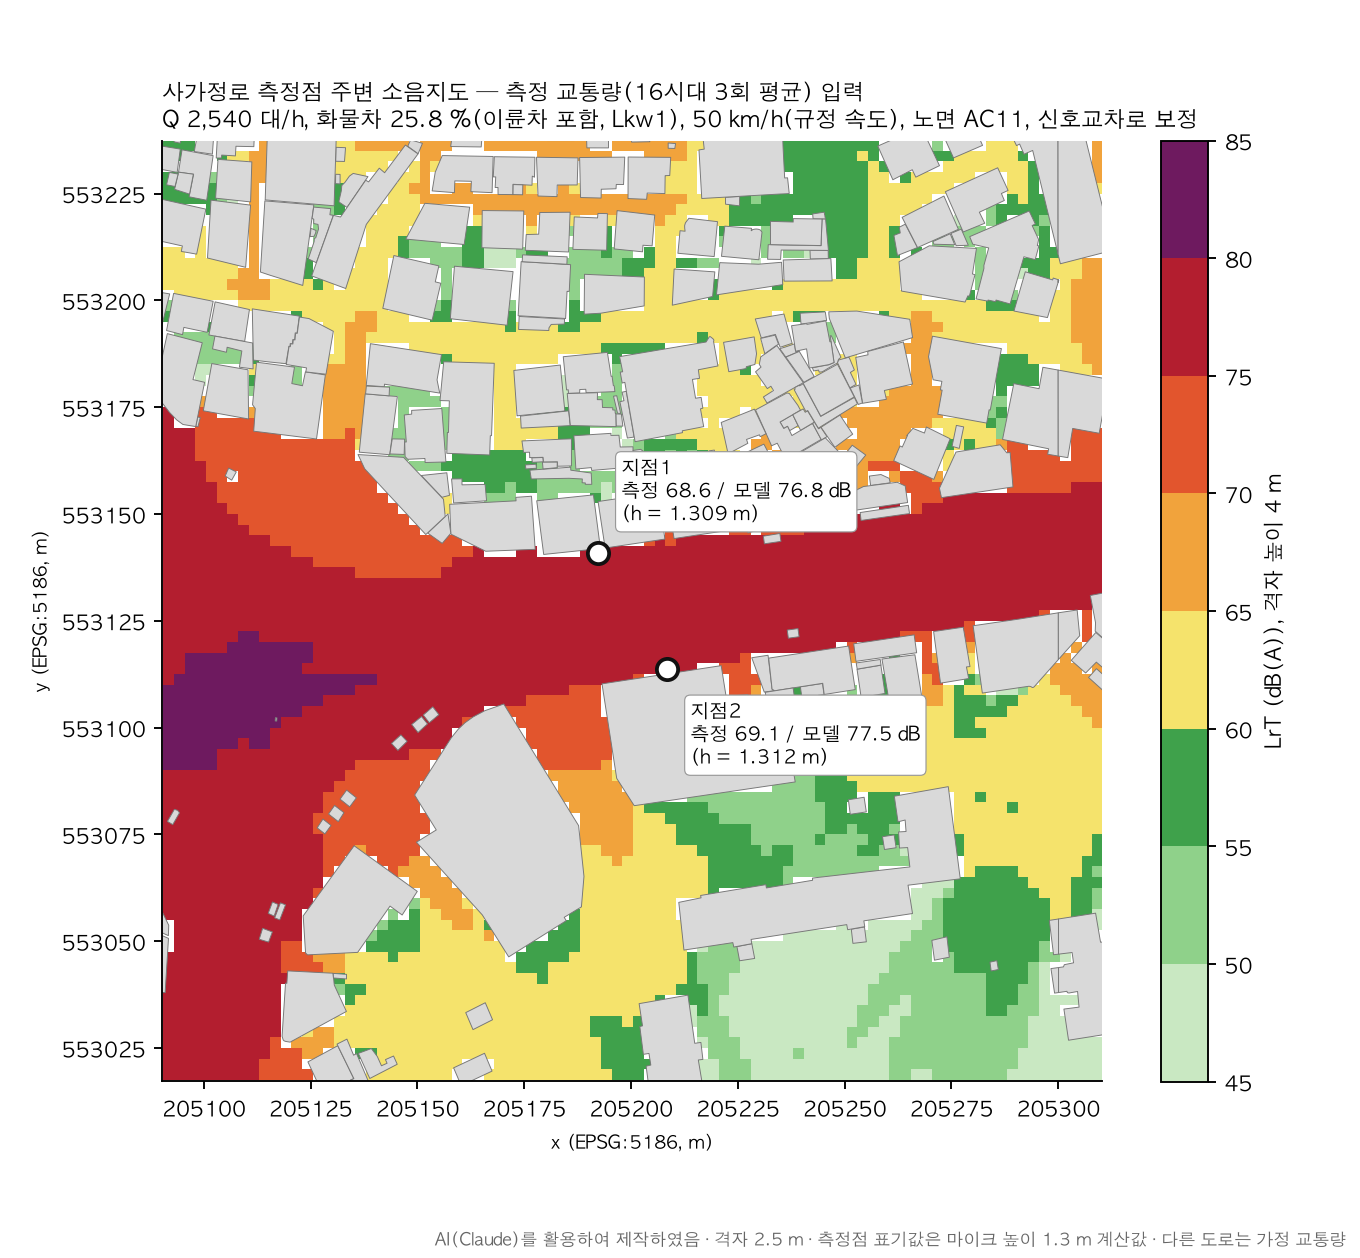
\includegraphics[width=0.78\linewidth]{소음지도_측정점주변_AVG.png}
\caption{측정점 위치(EPSG:5186 좌표)와 주변 계산 소음도(측정 교통량 3회 평균, 50 km/h, 격자 높이 4 m). 지점1 (205192.18, 553140.81), 지점2 (205208.36, 553113.68). 수음점 위치는 수치지도의 보도 경계와 현장에서 잰 도로끝선·건물 거리로 정했다. GPS 기록은 소수 셋째 자리(약 $\pm$50 m)까지만 있어 쓰지 않았다}
\end{figure}

\subsection{측정점별 결과표}
\small
\begin{longtable}{C{0.16}C{0.13}C{0.13}C{0.13}C{0.10}C{0.10}C{0.25}}
\caption{측정점별 회차별 \Laeq{} (단위 dB(A), 10분 측정, 유효 측정만)}\\
\toprule
\hd{측정점} & \hd{1회} & \hd{2회} & \hd{3회} & \hd{N1} & \hd{N2} & \hd{낮 산술평균 (에너지평균)} \\ \midrule
\endhead
\bottomrule
\endlastfoot
지점1 & 68.1 & 68.3 & 69.2 & \NA & \NA & 68.5 (68.6) \\ \midrule
지점2 & 68.9 & 69.0 & 69.3 & \NA & \NA & 69.1 (69.1) \\
\end{longtable}
\normalsize
\small
\begin{longtable}{C{0.10}C{0.11}C{0.11}C{0.11}C{0.11}C{0.11}C{0.11}L{0.24}}
\caption{측정점별 통계 지표(dB(A), 3회 산술평균, 기기 저장값). $L_{\mathrm{Amax}}$ 괄호 안은 3회 중 최댓값}\\
\toprule
\hd{측정점} & \hd{\Laeq} & \hd{$L_{\mathrm{Amax}}$} & \hd{$L_{\mathrm{Amin}}$} & \hd{$L_{10}$} & \hd{$L_{50}$} & \hd{$L_{90}$} & \hd{비고} \\ \midrule
\endhead
\bottomrule
\endlastfoot
지점1 & 68.5 & 82.7 (85.4) & 57.0 & 71.9 & 66.6 & 61.4 & 100 ms 자료로 다시 계산한 값과 0.04 dB 이내로 같다 \\ \midrule
지점2 & 69.1 & 83.8 (85.1) & 55.5 & 72.3 & 66.9 & 60.3 & $L_{\mathrm{Amax}}$와 $L_{\mathrm{Amin}}$은 기기값만 있다(1 s 저장) \\
\end{longtable}
\normalsize
{\small 회차별 값은 부록 E에 있다. 표준편차(회차 간)는 지점1 0.59 dB, 지점2 0.21 dB다. 같은 시각의 지점 간 차이(지점1 $-$ 지점2)는 $-$0.8, $-$0.7, $-$0.1 dB다. 두 기기의 교정 편차를 생각하면 1 dB 미만의 차이는 해석하지 않는다.\par}

\subsection{시간대별 변화}
측정은 16시대 한 시간 안에서만 했다. 그래서 하루 중 시간대별 변화는 알 수 없다. 아래 그림은 회차별 \Laeq 와 같은 시각의 교통량이다.
\begin{figure}[H]
\centering
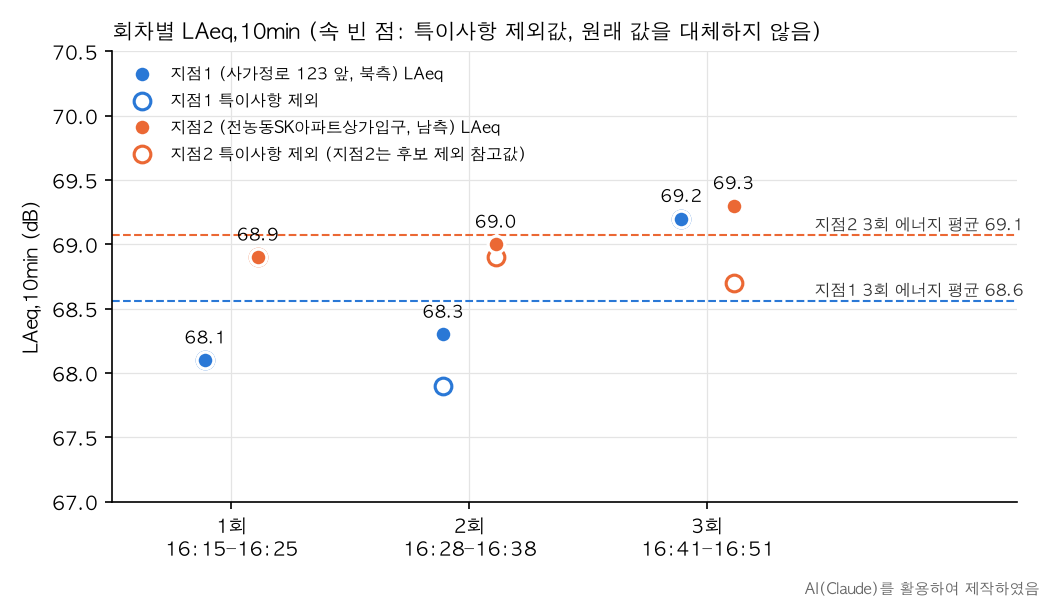
\includegraphics[width=0.62\linewidth]{지점별_LAeq_비교.png}\par\vspace{2mm}
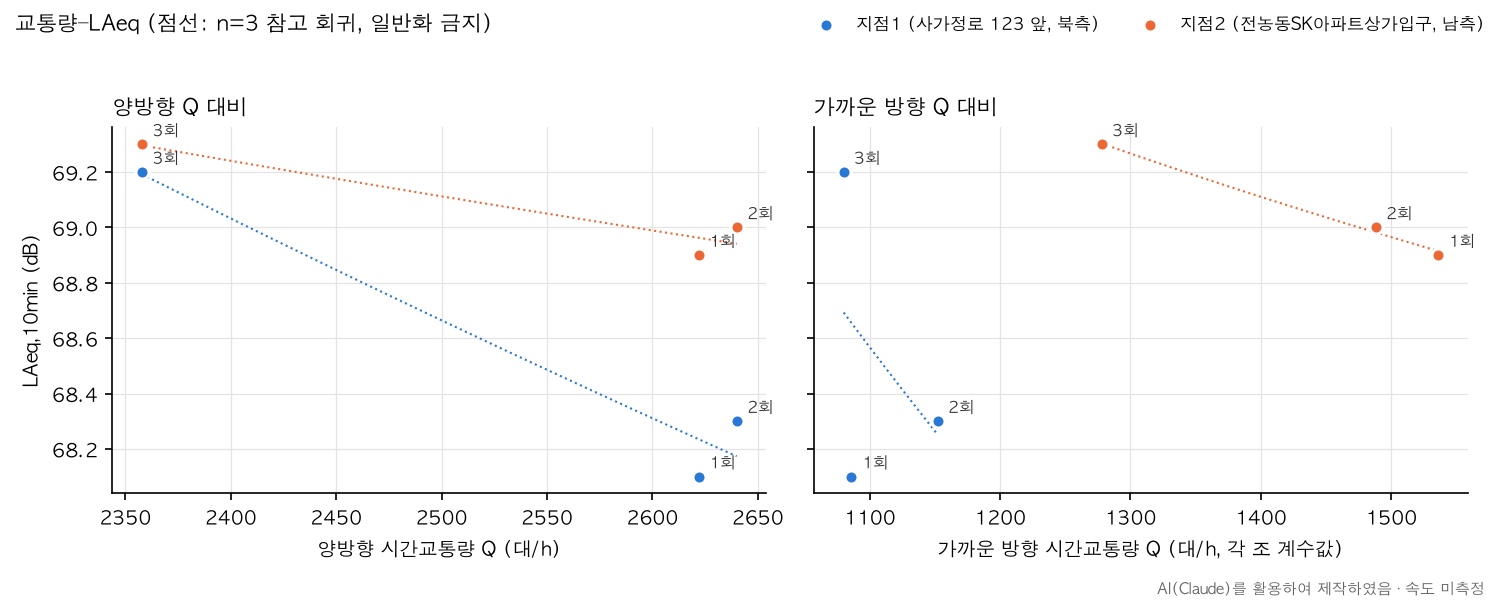
\includegraphics[width=0.95\linewidth]{교통량_LAeq_산점도.png}
\caption{회차별 \Laeq(위)와 시간당 교통량 대비 \Laeq(아래). $n=3$이고 \Laeq 변동 폭이 1 dB 정도라, 교통량과의 관계는 해석하지 않는다}
\end{figure}

\clearpage\subsection{동시 교통량·기상}
\footnotesize
\begin{longtable}{C{0.08}L{0.30}C{0.11}C{0.15}C{0.10}C{0.12}C{0.14}}
\caption{회차별 사가정로 교통량(10분 계수 $\times$ 6, 대/h). 화물차에 이륜차 포함}\\
\toprule
\hd{회차} & \hd{방향(계수 조)} & \hd{승용차} & \hd{화물차(이륜차 포함)} & \hd{합계} & \hd{화물차 비율} & \hd{평균 속도} \\ \midrule
\endhead
\bottomrule
\endlastfoot
1 & 상행(서행, 지점1 조) & 888 & 198 & 1086 & 18.2 \% & \NA \\
  & 하행(동행, 지점2 조) & 1080 & 456 & 1536 & 29.7 \% & \NA \\
  & \textbf{양방향} & 1968 & 654 & \textbf{2622} & 24.9 \% & \NA \\ \midrule
2 & 상행 & 828 & 324 & 1152 & 28.1 \% & \NA \\
  & 하행 & 1080 & 408 & 1488 & 27.4 \% & \NA \\
  & \textbf{양방향} & 1908 & 732 & \textbf{2640} & 27.7 \% & \NA \\ \midrule
3 & 상행 & 798 & 282 & 1080 & 26.1 \% & \NA \\
  & 하행 & 978 & 300 & 1278 & 23.5 \% & \NA \\
  & \textbf{양방향} & 1776 & 582 & \textbf{2358} & 24.7 \% & \NA \\ \midrule
평균 & \textbf{양방향} & 1884 & 656 & \textbf{2540} & 25.8 \% & \NA \\
\end{longtable}
\normalsize
{\small 상행·하행은 지도 기준으로 판정했다. 도로명주소 번지로 보면 지점1은 북측이고 그쪽 가까운 차로가 서쪽(도심) 방향이다. 원자료 폴더 이름은 이와 반대로 붙어 있다. 각 조는 자기 쪽 가까운 차로를 셌다. 전농로 등 다른 도로는 계수하지 않았다.\par}
\small
\begin{longtable}{C{0.10}C{0.12}C{0.10}C{0.11}C{0.10}C{0.22}C{0.25}}
\toprule
\hd{관측 시각} & \hd{풍속(m/s)} & \hd{풍향} & \hd{기온(°C)} & \hd{습도(\%)} & \hd{날씨·노면} & \hd{신호 주기(s)} \\ \midrule
\endhead
\bottomrule
\endlastfoot
16:00 & 2.5 & 남 & 16.1 & 30 & 맑음, 운량 0. 노면 건조 추정(당일 강수 기록 없음) & \NA \\ \midrule
17:00 & 1.3 & 서 & 15.2 & 31 & 맑음, 운량 0 & \NA \\
\end{longtable}
\addtocounter{table}{-1}
\normalsize
{\small 출처: 기상청 서울 관측소(ASOS 108, 종로구 송월동, 현장에서 서쪽으로 약 8 km) 매시 관측값(기상청 날씨누리 도시별관측, 2026-10-22 16:00·17:00, 2026-10-28 조회). 측정 시간(16:15--16:51)은 두 관측 시각 사이다. 현장에서 실측한 값이 아니다. 측정 당일 현장 기록에 적힌 인근 기상정보(네이버 지도 날씨: 풍속 1.8 m/s, 기온 15 °C)는 관측소 값과 조금 다르다. 보고서에서는 관측소 값을 쓴다. 신호 주기는 측정하지 않았다.\par}

%% ------------------------------------------------------------------
\section{기준 비교 평가(목적 가)}
\subsection{적용 지역 구분과 기준값}
용도지역은 토지이음(eum.go.kr) 토지이용계획 열람으로 확인했다(2026-10-28). 지점1 앞 필지(사가정로 123 = 전농동 38-97)는 \textbf{근린상업지역}이고, 지점2 앞 필지(사가정로 148 = 전농동 10, 전농동SK아파트)는 \textbf{제3종일반주거지역}이다. 두 측정점은 사가정로 도로끝선에서 3--4 m 떨어져 있어, 도로단에서 `차선수 $\times$ 10 m' 안의 도로변지역이다(ES 03301.1c 5.1.1 주 1). 학교·병원 등 부지경계 50 m 이내 여부는 토지이용계획으로 정할 수 없어 미확인이다. 토지이용계획에는 교육환경보호구역이 표시되어 있다. 지점1 필지는 상대보호구역만 해당하고, 지점2 필지(면적 72,275 m\textsuperscript{2})는 상대·절대보호구역이 함께 걸쳐 있다. 지점2는 ``가''지역이 되어도 도로변 기준값이 ``나''와 같다(65/55, 별표 11은 어차피 가목). 그래서 판정이 바뀌지 않는다. 지점1은 학교 등 부지경계 50 m 안이면 ``가''지역(65/55)·가목(68/58)으로 바뀌므로, 아래 판정에 이 조건을 함께 적었다.
\needspace{9\baselineskip}
\footnotesize
\begin{longtable}{C{0.09}C{0.14}C{0.10}C{0.17}C{0.14}C{0.18}C{0.18}}
\toprule
\hd{측정점} & \hd{용도지역} & \hd{50 m 규정} & \hd{별표 1 구분} & \hd{별표 1 기준 낮/밤} & \hd{별표 11 구분} & \hd{별표 11 기준 주간/야간} \\ \midrule
\endhead
\bottomrule
\endlastfoot
지점1 & 근린상업지역 & 미확인(상대보호구역 해당) & 도로변 ``다'' & 70 / 60 & 나목 & 73 / 63 \\ \midrule
지점2 & 제3종일반주거지역 & 미확인(판정 불변) & 도로변 ``가 및 나'' & 65 / 55 & 가목 & 68 / 58 \\
\end{longtable}
\addtocounter{table}{-1}
\normalsize

\subsection{소음 환경기준 비교}
\footnotesize
\begin{longtable}{C{0.09}C{0.12}C{0.15}C{0.18}C{0.10}C{0.10}C{0.08}C{0.18}}
\caption{측정소음도(산술평균, 정수)와 환경기준 비교(dB(A)) --- 참고 평가}\\
\toprule
\hd{측정점} & \hd{낮 측정소음도} & \hd{낮 기준} & \hd{낮 판정} & \hd{밤 측정소음도} & \hd{밤 기준} & \hd{밤 판정} & \hd{횟수 충족} \\ \midrule
\endhead
\bottomrule
\endlastfoot
지점1 & 69 (68.5) & 70(다) & 기준 이하(1 dB 아래)\newline 50 m 안이면 +4 초과 & \NA & 60 & 평가 불가 & 미충족(낮 3회, 13분 간격) \\ \midrule
지점2 & 69 (69.1) & 65(가 및 나) & \textbf{+4 초과} & \NA & 55 & 평가 불가 & 미충족(낮 3회, 13분 간격) \\
\end{longtable}
\normalsize

\subsection{교통소음 관리기준(도로) 비교}
\small
\begin{longtable}{C{0.10}C{0.18}C{0.30}C{0.14}C{0.28}}
\toprule
\hd{구분} & \hd{대상 지점} & \hd{측정소음도(지점별 산술평균의 산술평균)} & \hd{기준} & \hd{판정} \\ \midrule
\endhead
\bottomrule
\endlastfoot
주간 & 지점1, 지점2 & (68.5 + 69.1) / 2 = 68.8 → \textbf{69}\newline(ES 03304.1d 7.1.1.2) & 68(가, 지점2 쪽)\newline 73(나, 지점1 쪽) & 주거지역 쪽(가목) \textbf{+1 초과}, 상업지역 쪽(나목) 기준 이하 --- 참고 평가 \\ \midrule
야간 & --- & \NA & 58 / 63 & 평가 불가 \\
\end{longtable}
\addtocounter{table}{-1}
\normalsize

\subsection{평가 의견}
\begin{itemize}
\item 두 지점의 낮 측정소음도는 69 dB(A)로 같다. 회차 간 변동은 1.1 dB 이하로 작다. 도로 남측 지점2(제3종일반주거지역)는 환경기준(도로변 ``나'' 65)을 \textbf{4 dB} 넘고, 도로 관리기준(가목 68)을 \textbf{1 dB} 넘는다. 도로 북측 지점1(근린상업지역)은 환경기준(도로변 ``다'' 70)과 관리기준(나목 73) 모두 이하다. 다만 지점1이 학교 등 부지경계 50 m 안이면 기준이 65·68로 바뀌어 지점2와 같이 초과가 된다(미확인).
\item 도로 관리기준은 ES 03304.1d 7.1.1.2에 따라 두 지점을 평균한 하나의 측정소음도(69)로 평가했다. 그런데 두 지점은 별표 11 구분이 다르다(지점1 나목, 지점2 가목). 공정시험기준에는 이 경우의 처리 규정이 없다(원문에서 찾지 못함). 그래서 구분별 기준을 함께 적었다.
\item 측정은 평일 16시대에 10분씩 3회, 13분 간격으로 했다. 공정시험기준의 측정 횟수·간격 요건(환경기준: 낮 2시간 이상 간격 4회, 도로교통: 4시간 이상 간격 2회)을 채우지 못했다. 그래서 위 판정은 법정 평가가 아니라 \textbf{참고 평가}다.
\item 밤(22--06시)과 야간은 측정하지 않아 \textbf{평가 불가}다. 측정하지 않은 값을 모델값이나 추정값으로 채우지 않았다.
\item 지점2는 상가 입구 앞이다. 그래서 도로교통 측정점 요건(피해가 예상되는 거주 건물 경계)을 충족하는지는 미확인이다.
\item 이상 소음(사이렌, 경적, 오토바이)을 빼도 3회 평균은 0.0--0.3 dB만 낮아진다. 판정에는 영향이 없다.
\end{itemize}

%% ------------------------------------------------------------------
\clearpage\section{시뮬레이션 비교(목적 나)}
\subsection{비교 조건}
\footnotesize
\begin{longtable}{L{0.24}L{0.76}}
\toprule
\hd{항목} & \hd{내용} \\ \midrule
\endhead
\bottomrule
\endlastfoot
모델 버전·설정 파일 & 소음지도 소프트웨어 SORI v0.1(RLS-19 + ISO 9613-2). 점 계산은 커밋 7b02e79 기준이고, 6.8절 소음지도·3D 뷰어는 이름 변경(noisemap → SORI) 뒤 커밋 227dac7로 만들었다. 두 커밋의 계산식과 결과값은 같다. 시나리오별 설정은 field\_measurement/2026-10-22/model/\{R1,R2,R3,AVG\}\_v\{30,40,50\}/config.yaml에 있다. 재실행 명령은 scripts/run\_all.sh다 \\ \midrule
입력 교통량 & 사가정로에는 회차별 동시 계수값(10분 $\times$ 6)을 넣었다: R1 2622, R2 2640, R3 2358 대/h. AVG는 3회 평균 2540 대/h다. 방향 비율(하행 54.2--58.6 \%)도 실측값을 썼다. 계수하지 못한 도로는 가정값이다: 전농로 2331, 답십리로 1813, 서울시립대로 1554 대/h. 이 값은 기준선의 가정 일교통량(DTV 45,000, 35,000, 30,000 대/일, baseline/traffic.csv `가정값(실측 아님)')에 서울 주간 계수 0.0518을 곱한 것이다(model/*/traffic.csv의 note 열). 가정 DTV 자체의 산정 근거는 저장소에 기록되어 있지 않다(근거 미기록). 이 도로들이 측정점 레벨에 기여하는 정도는 0.3--0.5 dB다 \\ \midrule
계수 차종 → Pkw/Lkw1/Lkw2 & 승용차는 Pkw, 화물차(이륜차 포함)는 전부 Lkw1로 넣었고 Lkw2는 0이다. RLS-19는 이륜차를 Lkw2로 다룬다. 이륜차 대수가 따로 기록되지 않아 그렇게 나누지 못했다(민감도 \ref{sec:cause}) \\ \midrule
속도 & 사가정로는 30, 40, 50 km/h 세 시나리오로 계산했다. \textbf{기본은 규정 속도 50 km/h}다(OSM maxspeed 50, 안전속도 5030). 실제 속도는 미측정이다. 다른 도로는 50 km/h로 넣었다 \\ \midrule
노면·교차로 & 노면은 AC11(밀입도 아스팔트콘크리트)로 가정했다. 현장 노면은 미확인이다. 교차로 보정은 가장 가까운 신호교차로 기준으로 했다(dk\_rule: nearest\_signal). 측정점에서 15 m 안의 사가정로 음원에 붙는 $D_K$는 지점1 +0.5--1.0 dB, 지점2 +0.2--0.8 dB다(model/AVG\_v50/output/sources.csv). 그 결과 측정점 계산값은 지점1 +0.70--0.72 dB, 지점2 +0.52--0.53 dB 높아진다(results/모델\_측정\_비교.csv, 기본 판정 대비) \\ \midrule
수음점 위치·높이 & 측정점과 같은 좌표·높이의 점 수음점이다(4.1, 높이 1.309·1.312 m). 자기 벽면 반사도 포함했다(2차 반사까지). 계산 방법과 해석·가정 설정은 \ref{sec:method}·\ref{sec:assume}절에 있다 \\ \midrule
기상·전파 & 기온 15 °C, 습도 70 \%(코드 기본값). 관측값은 15.2--16.1 °C, 습도 30--31 \%다. 500 Hz 대기흡음 차이는 측정점 거리(4--30 m)에서 0.02 dB 미만이다(추정) \\ \midrule
측정값 평균 & 회차별 비교에는 각 회차의 10분 \Laeq 를 썼다. 시간대 비교에는 3회의 에너지평균(지점1 68.6, 지점2 69.1)을 썼다 \\ \midrule
이상 소음 구간 처리 & 원래 \Laeq 를 썼다(3.3). 제외값과의 차이는 0.6 dB 이하다 \\ \midrule
판정 기준 & 소음지도의 작성방법 별표 2 제15호: 오차 평균 $\pm$3 dB 이내, 표준편차 3 이하(원칙). 지점별 차이가 $\pm$5 dB 이상이면 원인을 분석한다 \\ \midrule
비교 단위 & 측정점 2 $\times$ 회차 3 = 6개(회차별 동시 교통량으로 계산). 측정점별 시간대 값(3회 평균)도 함께 적었다 \\
\end{longtable}
\addtocounter{table}{-1}
\normalsize

\subsection{계산 방법(RLS-19 방출 + ISO 9613-2 전파)}\label{sec:method}
계산 방법은 소프트웨어 기술 노트(TECHNICAL\_NOTES.md 1--3·6절)를 요약했다. 도로 음원의 방출은 RLS-19로 계산하고, 음원에서 수음점까지의 전파는 ISO 9613-2로 계산한다.

\textbf{계산 흐름.}
\begin{enumerate}
\item \textbf{입력 준비:} 수치지도(건물, 도로, 등고선, 표고점)로 지형 DTM(1 m), DSM, 지면계수 $G$ 래스터를 만든다.
\item \textbf{음원 구성:} 도로 위상으로 교차로를 판정한 뒤, 방향별 음원선을 RLS-19 그림 6(Bild 6) 규칙으로 배치한다. 음원선은 짧은 구간으로 나누고, 구간마다 음원선 음향파워레벨 $L_W'$를 RLS-19 식 (4)--(9)로 계산한다.
\item \textbf{수음점 계산:} 각 수음점에서 직접음과 1·2차 허상음원(반사음) 경로마다 수직단면을 만들고 아래 식으로 합산한다.
\end{enumerate}
\begin{equation*}
L = 10\lg\sum_{\text{구간·경로}} 10^{0.1\,(L_W - A + D_c)}, \qquad A = A_{\mathrm{div}} + A_{\mathrm{atm}} + A_{\mathrm{gr}} + A_{\mathrm{bar}}, \qquad L_W = L_W' + 10\lg l
\end{equation*}

\textbf{두 기준의 결합 근거.} RLS-19는 차량 음향파워를 반공간($\Omega = 2\pi$) 방사로 정의한다. ISO 9613-2는 자유공간 점음원($A_{\mathrm{div}} = 20\lg d + 11$)에 지면효과 $A_{\mathrm{gr}}$를 더한다. 일반법(7.3.1)에서 단단한 지면($G=0$)이고 $d_p \le 30(h_s+h_r)$이면($q=0$) $A_{\mathrm{gr}} = -3$ dB다. 그러면 $L = L_W - 10\lg(2\pi d^2)$가 되어(차이 0.02 dB) RLS-19의 반공간 정의와 일치한다. 따라서 구간 음향파워 $L_W = L_W' + 10\lg l$을 ISO 식 (3)의 $L_W$로 그대로 쓰고, 일반법에서는 $D_c = 0$으로 둔다. 이 일치는 $q = 0$ 범위에서만 성립한다. $d_p > 30(h_s+h_r)$이면 $q = 1 - 30(h_s+h_r)/d_p$이고 $A_m = -3q(1-G_m)$이라(ISO 표 3), $G = 0$에서 $A_{\mathrm{gr}}$은 $-3$ dB보다 작아져 최대 $-6$ dB까지 간다. 경계 거리는 측정점(높이 1.3 m)에서 54 m, 격자(4 m)에서 135 m다. RLS-19 자체 전파식은 지면 감쇠를 $D_{gr} = \max\{4.8 - (h_m/s)(34 + 600/s);\,0\} \ge 0$으로 두므로(원문 식 14), 단단한 지면의 먼 음원은 이 결합에서 RLS-19 자체 식보다 높게 계산된다. 직선 선음원 해석해 시험(0.05 dB 이내)은 수음 높이 4 m, $d_p \le 108$ m로 $q = 0$ 범위만 확인한 것이다. 이 영향의 크기는 표 \ref{tab:ground}에 있다.

\footnotesize
\begin{longtable}{L{0.22}L{0.30}L{0.48}}
\caption{원문 식과 구현의 대응, 이번 계산의 설정}\label{tab:impl}\\
\toprule
\hd{원문} & \hd{내용} & \hd{구현(함수)과 이번 계산의 설정} \\ \midrule
\endhead
\bottomrule
\endlastfoot
RLS-19 식 (4)--(6), 표 3 & 음원선 $L_W'$, 차종별 $L_W$ & \texttt{rls19.LW\_prime}, \texttt{LW\_vehicle}. Pkw·Lkw1·Lkw2별 속도를 따로 넣을 수 있고, 30 km/h 하한을 둔다 \\ \midrule
RLS-19 표 4a·4b & 노면 보정 $D_{SD}$ & \texttt{rls19.D\_SD}. 이번 계산은 AC11(설정 \texttt{surface\_map}) \\ \midrule
RLS-19 식 (7a--c) & 종단경사 $D_{LN}$ & \texttt{rls19.D\_LN}. 경사는 평활 DTM(가우스 $\sigma$ 5 m)에서 도로를 따라 30 m 구간으로 구한다 \\ \midrule
RLS-19 식 (8), 표 5 & 교차로 보정 $D_K$ & \texttt{rls19.D\_K}. 기준 교차점은 \texttt{dk\_rule: nearest\_signal}(\ref{sec:assume}절 표의 13번, 원문 문언과 다름) \\ \midrule
RLS-19 식 (9), 3.3.8 & 다중반사 할증 $D_{\mathrm{refl}}$ & \texttt{rls19.D\_refl}. 도로를 향한 평행 파사드(각도 차 5° 이내)가 있을 때 적용한다. 명시적 반사(ISO 7.5)와 함께 적용한다(RLS-19 3.3.8, 3.6) \\ \midrule
RLS-19 3.2, 3.3.1, 그림 6 & 음원 높이, 구간 분할, 음원선 위치 & \texttt{build.build\_sources}, \texttt{lane\_layout}, \texttt{source\_offsets}. 음원 높이는 지면 + 0.5 m다. 구간 길이는 간선 3 m, 이면도로 5 m다 \\ \midrule
RLS-19 3.3.2 & 방향별 교통량 & 실측 하행 비율(0.542--0.586)을 사가정로 측정 구간에 지정했다(\texttt{dir\_split\_fwd}) \\ \midrule
ISO 9613-2 식 (7) & 기하 확산 $A_{\mathrm{div}}$ & \texttt{iso9613.A\_div} \\ \midrule
ISO 9613-2 식 (8), 표 2 / ISO 9613-1 & 대기 흡음 $A_{\mathrm{atm}}$ & \texttt{iso9613.A\_atm}. 흡음계수 $\alpha$는 ISO 9613-1로 계산한다(15 °C, 70 \%, 101.325 kPa) \\ \midrule
ISO 9613-2 식 (9), 표 3 & 지면 효과 $A_{\mathrm{gr}}$(일반법) & \texttt{iso9613.A\_gr\_general}. 지면계수는 전역 $G = 0$이다(다공성 지면 폴리곤 미입력). $q > 0$ 영역의 $A_m = -3q(1-G_m)$도 원문대로 계산한다 \\ \midrule
ISO 9613-2 식 (12), (14)--(18) & 차폐 $A_{\mathrm{bar}}$, $D_z$, $C_3$, $K_{\mathrm{met}}$ & \texttt{iso9613.D\_z}, \texttt{path\_loss}. $C_2 = 20$이다. $D_z$ 상한은 단일 회절 20 dB, 이중 회절 25 dB다 \\ \midrule
ISO 9613-2 7.5, 식 (19)(20), 표 4 & 반사(허상음원), 반사 크기 조건 & \texttt{solver.compute}. 반사계수는 $\rho = 0.8$이다. 점 수음점은 2차 반사까지 계산한다 \\ \midrule
ISO 9613-2 1절 비고 1 & A가중 단일값 계산 & 500 Hz 감쇠항 한 대역으로 계산한다 \\
\end{longtable}
\normalsize

\footnotesize
\begin{longtable}{L{0.34}C{0.11}C{0.11}C{0.11}L{0.33}}
\caption{지면 감쇠 처리에 따른 계산값 변화(3회 평균 교통량, 50 km/h, dB). results/지면효과\_진단.csv}\label{tab:ground}\\
\toprule
\hd{조건} & \hd{지점1} & \hd{지점2} & \hd{지점2(P2c)} & \hd{격자(4 m)·벽면, 기준 대비} \\ \midrule
\endhead
\bottomrule
\endlastfoot
기준: 일반법, $G = 0$, $q$ 항 포함 & 76.77 & 77.51 & 77.96 & --- \\ \midrule
$q$ 항 제거(진단용 사본) & $-$0.20 & $-$0.13 & $-$0.12 & 격자 중앙값 $-$0.01, 5 \% $-$0.10, 최소 $-$1.21. 벽면 중앙값 0.00, 최소 $-$1.19 \\ \midrule
대안법(ISO 식 10 = RLS-19 식 14 형태, $D_\Omega$ 포함) & $-$1.90 & $-$1.49 & $-$1.36 & 격자 중앙값 $-$0.70, 5--95 \% $-$2.23--+1.98 \\
\end{longtable}
\normalsize
{\small 대안법은 RLS-19 자체 지면 감쇠와 같은 식이지만, 차폐가 있을 때의 결합 방식(ISO 식 12, RLS-19 식 11의 $\max\{D_{gr}; D_z\}$)은 같지 않다. 그래서 격자에서 일부 차폐 지점은 오히려 높아진다. 진단용 사본은 저장소 코드를 바꾸지 않고 \texttt{q}만 0으로 고정한 복사본이다(scripts/ground\_diag.py).\par}
\textbf{검증.} 2026-10-27에 저장소 시험 44개(\texttt{python -m pytest -q tests})를 다시 실행했고 모두 통과했다. 시험 대상은 다음과 같다.
\begin{itemize}
\item 원문 식 재계산($L_{W0}$, $L_W'$, $D_K$, $D_{\mathrm{refl}}$, $D_{LN}$, $D_{SD}$)
\item 대기흡음계수 $\alpha$(ISO 9613-2 표 2 대조, 1 \% 이내)
\item $A_{\mathrm{gr}}$, $D_z$ 수계산
\item 점음원 자유음장
\item 직선 선음원 해석해(0.05 dB 이내, 수음 높이 4 m·$d_p \le 108$ m로 $q = 0$ 범위만)
\item 얇은 벽 단일 회절, 1·2차 반사 수계산
\item 교차로 판정과 \texttt{dk\_rule}
\end{itemize}
이번 측정점에서는 모델 직접음을 손계산과 비교했고 0.2 dB 이내로 맞았다.

다만 원문 식 재계산 시험은 원문 수치표와 대조한 것이 아니다. 같은 식을 다시 계산한 자기 일관성 확인이다. RLS-19 공식 시험과제(TEST-20, DIN/TR 8999-1)와는 아직 비교하지 않았다.

\subsection{원문이 명확하지 않은 사항의 해석·가정 설정}\label{sec:assume}
원문에 값이 없거나 해석이 필요한 항목을 이번 계산에서 어떻게 설정했는지 정리했다(TECHNICAL\_NOTES.md 4·5·5a절). 판정은 네 가지로 구분했다.
\begin{itemize}
\item \textbf{원문}: 원문 규정 그대로
\item \textbf{해석}: 원문의 원칙에서 이끌어 낸 것
\item \textbf{미확인 가정}: 자료로 확인하기 전의 가정
\item \textbf{가정값}: 근거 수치 자체가 가정
\end{itemize}
영향 크기는 별도 표시가 없으면 전농사거리 모델에서 잰 값이다.
\footnotesize
\begin{longtable}{C{0.04}L{0.15}L{0.33}C{0.11}L{0.37}}
\caption{해석·가정 설정과 영향}\label{tab:assume}\\
\toprule
\hd{\#} & \hd{항목} & \hd{이번 계산의 설정} & \hd{판정} & \hd{근거·영향} \\ \midrule
\endhead
\bottomrule
\endlastfoot
1 & 주파수 대역 & 500 Hz 한 대역(A가중 단일값) & 원문 & RLS-19는 A가중 단일값만 준다. ISO 9613-2 1절 비고 1에 따랐다 \\ \midrule
2 & 기상 조건 & 순풍 조건($L_{AT}(DW)$). 장기 기상보정 $C_{\mathrm{met}}$는 적용하지 않는다 & 해석 & RLS-19 평가레벨과 같은 조건이다. 측정점은 음원에서 4--30 m라 $C_{\mathrm{met}}$가 0에 가깝다(추정) \\ \midrule
3 & 지면 계수 & 일반법(7.3.1), 전역 $G = 0$ & 가정값 & 측정점 주변은 포장면이다. $q = 0$ 범위에서만 $A_{\mathrm{gr}} = -3$ dB로 RLS-19 반공간 정의와 일치한다. 먼 음원($q > 0$)은 RLS-19 자체 식보다 높게 계산된다. 측정점 영향은 $q$ 항 $-$0.1--$-$0.2 dB, RLS-19식 지면 처리 $-$1.5--$-$1.9 dB다(표 \ref{tab:ground}) \\ \midrule
4 & 대기 조건 & 15 °C, 70 \%, 101.325 kPa & 가정값 & 기상청 서울 관측값(15.2--16.1 °C, 30--31 \%, 1025.6--1025.8 hPa)과 기온은 비슷하지만 습도는 다르다. 거리가 짧아 영향은 작다(0.02 dB 미만, 추정) \\ \midrule
5 & 차폐 계산 & 수직단면의 상부 볼록껍질(고무줄법). 회절 모서리가 2개 이상이면 이중 회절로 계산한다. 측면 회절(ISO 식 13)과 가시선 위 장애물의 음($-$)의 $z$는 고려하지 않는다 & 해석 & 측정점은 도로가 직접 보여 차폐 영향이 없다(추정) \\ \midrule
6 & 반사 & $\rho = 0.8$(ISO 표 4 `창이 있는 건물 벽'). 2 m 미만 파사드 변은 뺀다. 2차 반사는 수음점 50 m 안에서 서로 마주 보는 면 쌍만 찾는다 & 가정값 & 측정점 뒤 벽 반사가 결과에 들어간다(지점1 1차 반사 성분 72.1 dB, 50 km/h, 3회 평균) \\ \midrule
7 & 다중반사 할증과 명시적 반사 & 둘 다 적용 & 원문 & RLS-19 3.3.8은 평행 반사면 사이 구간마다 할증을, 3.6은 1·2차 거울상 음원을 정한다. 함께 쓰지 말라는 규정은 원문에서 찾지 못했다. 측정점에서 $D_{\mathrm{refl}}$을 끄면 $-$0.15--$-$0.23 dB(표 \ref{tab:combo}) \\ \midrule
8 & 음원 높이의 지면 & 음원점 위치의 DTM + 0.5 m(\texttt{source\_ground: dtm\_at\_source}) & 원문(구현은 옵션) & 원문은 ``0,5 m über dem Boden''이다. 노면 고도 자료가 없어 DTM으로 대신했다 \\ \midrule
9 & 구간 길이 & 간선 3 m, 이면도로 5 m 고정. 경험칙 $l \le s/2$는 진단만 한다 & 해석 & 낮고 가까운 수음점(높이 1.5 m, 거리 2 m, 구간 5 m)에서 해석해와 최대 $\pm$0.54 dB 차이가 났다. 측정점(1.3 m, 도로끝선 3--4 m)에도 같은 크기의 오차가 있을 수 있다 \\ \midrule
10 & 음원선 위치 & 도로중심선을 방향 경계로 본다. 방향별 차로 수는 확인값이 없으면 $\lceil n/2\rceil$이다. 차로폭은 도로폭/차로수를 2.75--3.5 m로 제한한 값이다 & 미확인 가정·가정값 & 차로폭 3.0 m 고정과 비교하면 파사드 5--95 \%에서 $-$0.29--+0.20 dB 차이 난다. 홀수 차로 규칙을 바꾸면 $-$0.35--+0.25 dB(격자) 차이 난다 \\ \midrule
11 & 횡단경사 & 반영하지 않는다 & 해석 & 횡단경사 2 \%(가정값)를 넣으면 최고 레벨 파사드가 $-$0.02--$-$0.03 dB 달라진다 \\ \midrule
12 & 교차로 거리 $x$ & 음원선 교차점 대신 도로중심선 교차점까지 거리로 근사한다 & 해석 & 최대 약 0.25 dB \\ \midrule
13 & 교차로 보정 기준 교차점 & \texttt{nearest\_signal}: 소속 교차점 기준 값과 가장 가까운 신호·회전교차로 기준 값 중 큰 쪽 & 원문과 다름(옵션) & 원문 3.3.7은 $x$를 ``서로 교차하거나 접속하는 음원선의 가장 가까운 교점''까지 거리로 정한다. 원문대로면 기본 \texttt{nearest}가 맞다. 기본 \texttt{nearest}로 계산하면 가까운 이면도로 접속부(전농로14길) 때문에 측정점 부근 $D_K$가 0이 된다. 신호에 따른 가감속은 소도로 접속부와 관계가 없어 이 옵션을 택했다. 측정점 계산값 증가는 지점1 +0.70--0.72 dB, 지점2 +0.52--0.53 dB다(\ref{sec:cause}절) \\ \midrule
14 & 신호교차로 자동 판정 & 차로수 4 이상인 도로축 2개 이상이 만나면 신호교차로로 판정 & 가정값 & 전농사거리는 신호교차로로 판정된다 \\ \midrule
15 & 방향별 교통량 & 사가정로 측정 구간에 실측 비율 지정. 그 밖의 도로는 50:50 & 원문 & RLS-19 3.3.2: 조사 자료가 있으면 표준값 대신 사용한다 \\ \midrule
16 & 종단경사 & 등고선 DTM을 평활($\sigma$ 5 m)한 뒤 30 m 구간으로 구한다 & 가정값 & 자연지형 기준이라 깎거나 쌓은 도로의 실제 경사와 다를 수 있다. 사가정로 동측 고갯길이 해당할 수 있다(미확인) \\ \midrule
17 & 건물 높이 & 층수 $\times$ 3.0 m. 기저고는 외곽 정점 지형고의 최솟값 & 가정값 & 측정점 앞 직접음에는 영향이 없다. 반사 크기 조건에만 영향을 준다 \\ \midrule
18 & 차종·노면·속도 & 화물차(이륜차 포함)는 전부 Lkw1, 노면 AC11, 사가정로 30·40·50 km/h. 다른 도로는 50 km/h & 가정값 & 6.1절과 \ref{sec:cause}절. 차이의 가장 큰 요인이다 \\ \midrule
19 & 번역본과 원문 차이 & 식 (8)은 곱(KKT $\cdot$ max), 3.1은 올림(aufzurunden)으로 원문대로 구현했다 & 원문 & 국문 번역본 오류 2건 \\
\end{longtable}
\normalsize

\subsection{측정값과 계산값}
\small
\begin{longtable}{C{0.10}C{0.12}C{0.15}C{0.15}C{0.12}L{0.36}}
\caption{측정 \Laeq{}와 계산 \Laeq(모델 $L_{rT}$) 비교(dB(A), 차이 = 측정 $-$ 계산, 50 km/h)}\\
\toprule
\hd{측정점} & \hd{시간대} & \hd{측정 \Laeq} & \hd{계산 \Laeq} & \hd{차이} & \hd{비고(30 / 40 km/h일 때 차이)} \\ \midrule
\endhead
\bottomrule
\endlastfoot
지점1 & 낮(16시대) & 68.6 & 76.8 & $-$8.2 & $-$5.6 / $-$6.6 \\ \midrule
지점1 & 밤 & \NA & --- & 평가 불가 & 야간 교통량 미측정 \\ \midrule
지점2 & 낮(16시대) & 69.1 & 77.5 & $-$8.4 & $-$5.7 / $-$6.8 \\ \midrule
지점2 & 밤 & \NA & --- & 평가 불가 & 야간 교통량 미측정 \\
\end{longtable}
\normalsize

\subsection{차이 통계}
차이 $d_i = L_{\text{측정},i} - L_{\text{계산},i}$, 비교 수 $n$(측정점 2 $\times$ 회차 3). 평균 차이와 표준편차(표본)는 다음과 같다.
\begin{equation*} \bar d = \frac{1}{n}\sum_{i=1}^{n} d_i, \qquad s = \sqrt{\frac{\sum_{i=1}^{n}\left(d_i-\bar d\right)^2}{n-1}} \end{equation*}
\small
\begin{longtable}{L{0.20}C{0.14}C{0.14}L{0.32}L{0.20}}
\toprule
\hd{지표} & \hd{50 km/h(기본)} & \hd{30 km/h(참고)} & \hd{고시 기준(별표 2 제15호)} & \hd{판정(50 km/h)} \\ \midrule
\endhead
\bottomrule
\endlastfoot
비교 수 $n$ & 6 & 6 & --- & --- \\ \midrule
평균 차이 & $-$8.3 & $-$5.7 & $\pm$3 dB 이내(음수면 모델이 높게 계산) & \textbf{미충족} \\ \midrule
표준편차 & 0.65 & 0.67 & 3 이하 & 충족 \\ \midrule
최대 차이(절댓값) & 8.8 & 6.2 & $\pm$5 dB 이상이면 그 지점 원인 분석 & 두 지점 모두 원인 분석 대상(\ref{sec:cause}) \\
\end{longtable}
\addtocounter{table}{-1}
\normalsize
{\small 측정점이 2곳이라 측정점 사이의 공간 변동은 평가할 수 없다. 표준편차는 주로 회차에 따른 변동을 나타낸다. 또한 $n = 6$은 같은 회차의 두 지점이 교통량 입력을 공유하므로 독립 표본이 아니다. 따라서 표준편차 판정(3 이하)의 의미는 제한적이다. 회차 간 변화의 방향도 서로 다르다. 모델에서는 교통량이 가장 적은 3회가 가장 낮고, 측정에서는 3회가 가장 높다.\par}
\begin{figure}[H]
\centering
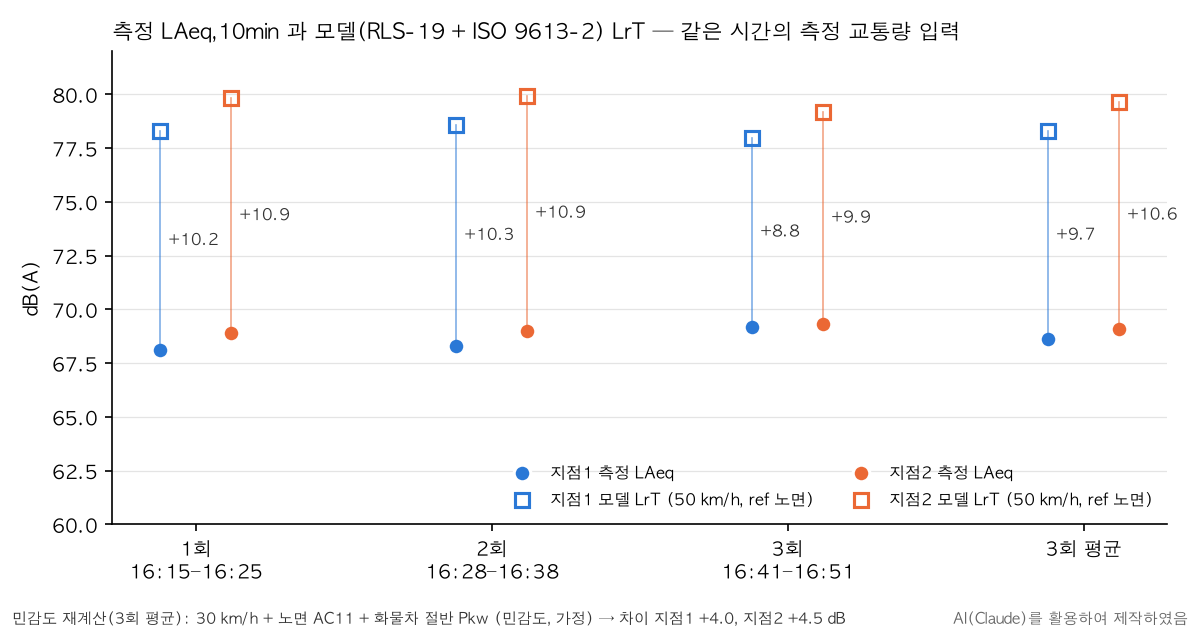
\includegraphics[width=\linewidth]{모델_측정_비교.png}
\caption{회차별 측정 \Laeq 와 모델 $L_{rT}$(30, 40, 50 km/h). 그림의 숫자는 측정 $-$ 모델이다(본문과 같은 부호)}
\end{figure}

\clearpage\subsection{차이 원인 검토}\label{sec:cause}
\footnotesize
\begin{longtable}{L{0.14}L{0.52}L{0.34}}
\toprule
\hd{검토 항목} & \hd{확인 내용} & \hd{영향 방향·크기(추정이면 `추정')} \\ \midrule
\endhead
\bottomrule
\endlastfoot
계산 검산 & 직접음 계산은 구현한 식과 일치한다(손계산과 0.2 dB 이내). 원문 수치표와 공식 시험과제(TEST-20, DIN/TR 8999-1)와의 대조는 하지 않았다. 따라서 구현이 원문과 같다는 것은 확인되지 않았다 & --- \\ \midrule
교통량 입력 & 사가정로는 동시 계수값과 일치시켰다. 다른 도로는 가정값이다 & 다른 도로 기여는 0.3--0.5 dB(계산) \\ \midrule
차종 구분 & 화물차 계수에 이륜차와 소형 화물차(3.5 t 이하 포함 가능)가 섞여 있다. 이를 전부 Lkw1로 넣었다 & 50 km/h·AC11 기준 실제 실행값: 화물차 절반 Pkw $-$1.07--$-$1.09, 전부 Pkw $-$2.49--$-$2.55, 전부 Lkw2 +1.62--+1.65 dB(표 \ref{tab:combo}) \\ \midrule
노면 & 현장 노면은 미확인이다. AC11로 넣었다(기본 매핑 대비 $-$2.2 dB) & 노면 가정에 따라 $\pm$2 dB 정도(추정) \\ \midrule
주행속도 & 미측정이다. 규정 속도 50 km/h로 넣었다. 측정점은 신호교차로 접근부(90--100 m)라 실제 평균 속도는 이보다 낮았을 가능성이 크다 & 50 → 30 km/h에서 $-$2.6 dB(계산) \\ \midrule
신호 대기 & RLS-19는 모든 차량이 같은 속도로 달린다고 본다. 정지·가감속은 식에 없다. 교차로 보정 $D_K$(신호교차로, 120 m 안)는 반영했다 & 정지 차량 비중만큼 모델이 높게 계산됨(추정) \\ \midrule
교차로 보정 & 가장 가까운 신호교차로 기준 $D_K$(\texttt{dk\_rule: nearest\_signal})를 적용했다. 기본 판정(\texttt{nearest})으로는 측정점 부근 $D_K$가 0이다. 원문 3.3.7은 $D_K$를 출발·제동에 따른 ``방해 효과(Störwirkung)''로 설명하고, 3.3.1은 이를 ``할증(Zuschlag)''으로 부른다. 측정 \Laeq 에 해당하는 음향 에너지 증가인지는 원문에 적혀 있지 않다(미확인). 또 \texttt{nearest\_signal}은 원문의 기준 교차점 정의와 다르다(표 \ref{tab:assume} 13번) & 모델을 높이는 쪽: 기본 판정 대비 지점1 +0.70--0.72, 지점2 +0.52--0.53 dB. $D_K$를 모두 끄면 지점1 $-$0.93, 지점2 $-$0.65 dB(표 \ref{tab:combo}) \\ \midrule
반사 & 지점1은 건물 벽 1.0 m 앞이고, 모델도 같은 위치에 벽 반사를 포함했다. 지점2는 수치지도의 도로끝선--건물 간격(6.25 m)이 현장(4.45 m)과 다르다 & 지점2 위치를 도로끝선 기준으로 바꾸면 계산값이 +0.4 dB 올라간다(계산). 이 보정은 지점2의 차이(측정 $-$ 계산)를 $-$8.4에서 $-$8.9 dB로 키운다(3회 평균, 50 km/h, 수음점 P2c) \\ \midrule
배경소음 & 사이렌, 경적, 오토바이 구간은 측정값을 높이는 쪽이다 & 0.0--0.6 dB(측정) \\ \midrule
기상 & 기상청 서울 관측값은 맑음, 16.1--15.2 °C, 습도 30--31 \%, 남풍 2.5 m/s(16시)에서 서풍 1.3 m/s(17시)다. 모델은 15 °C, 70 \%다. 수음점이 음원에서 4--30 m 거리라 기상 영향은 작다 & 작음(추정) \\ \midrule
기타 & RLS-19 방출식은 독일 차량·타이어 기준이라 보수적일 수 있다. 차도 쪽 주정차 차량이 마이크(1.3 m)를 가렸을 수도 있다 & 조합 실제 실행(표 \ref{tab:combo}): 30 km/h·절반 Pkw에서 차이 $-$4.3/$-$4.4 dB가 남는다(지점1/지점2). 이전 판의 ``약 +4.5 dB''는 이 조합의 근사였다. $D_K$·$D_{\mathrm{refl}}$까지 끄면 $-$3.1/$-$3.5, 화물차 전부 Pkw까지 가정하면 $-$1.3/$-$1.5 dB다 \\
\end{longtable}
\addtocounter{table}{-1}
\normalsize

%% ------------------------------------------------------------------
\clearpage\subsection{조합 민감도(실제 실행)}\label{sec:combo}
속도, 차종, 노면, $D_K$, $D_{\mathrm{refl}}$ 조합 96개를 모델로 각각 실행했다. 대표 조합은 표 \ref{tab:combo}와 같다.
\footnotesize
\begin{longtable}{L{0.52}C{0.12}C{0.12}C{0.12}C{0.12}}
\caption{조합 민감도 실제 실행 결과(3회 평균 교통량, 차이 = 측정 $-$ 모델, dB). 전체 96개 조합은 results/민감도\_조합.csv}\label{tab:combo}\\
\toprule
\hd{조건(바꾼 항목 외에는 기준과 같음)} & \hd{지점1 계산} & \hd{지점1 차이} & \hd{지점2 계산} & \hd{지점2 차이} \\ \midrule
\endhead
\bottomrule
\endlastfoot
기준: 50 km/h, 화물차 전부 Lkw1, AC11, $D_K$·$D_{\mathrm{refl}}$ 켬 & 76.77 & $-$8.21 & 77.51 & $-$8.45 \\ \midrule
$D_K$ 끔 & 75.84 & $-$7.29 & 76.86 & $-$7.80 \\
$D_{\mathrm{refl}}$ 끔 & 76.62 & $-$8.07 & 77.28 & $-$8.21 \\
$D_K$·$D_{\mathrm{refl}}$ 끔 & 75.68 & $-$7.13 & 76.62 & $-$7.56 \\ \midrule
노면 기본 매핑(아스팔트 → ref) & 79.01 & $-$10.46 & 79.75 & $-$10.69 \\
화물차 절반 Pkw & 75.70 & $-$7.14 & 76.42 & $-$7.35 \\
화물차 전부 Pkw & 74.28 & $-$5.72 & 74.96 & $-$5.89 \\
화물차 전부 Lkw2 & 78.39 & $-$9.83 & 79.16 & $-$10.09 \\ \midrule
30 km/h & 74.13 & $-$5.57 & 74.81 & $-$5.74 \\
30 km/h, 화물차 절반 Pkw & 72.85 & $-$4.29 & 73.48 & $-$4.41 \\
30 km/h, 화물차 절반 Pkw, $D_K$·$D_{\mathrm{refl}}$ 끔 & 71.69 & $-$3.14 & 72.54 & $-$3.47 \\
30 km/h, 화물차 전부 Pkw & 71.02 & $-$2.47 & 71.55 & $-$2.48 \\
30 km/h, 화물차 전부 Pkw, $D_K$·$D_{\mathrm{refl}}$ 끔 & 69.80 & $-$1.25 & 70.57 & $-$1.51 \\
\end{longtable}
\normalsize
{\small 각 조합은 모델을 따로 실행한 값이다(단순 합산 아님, scripts/sensitivity\_combo.py). 측정값은 3회 에너지평균(지점1 68.56, 지점2 69.07 dB)이다. 96개 조합의 차이 범위는 $-$12.2--$-$1.3 dB이고, 고시 기준($\pm$3 dB) 안에 드는 것은 30·40 km/h에 화물차 전부 Pkw를 가정한 9개 값뿐이다. 차종 가정의 50 km/h 효과는 이전 판의 근사($-$1.1, $-$2.6, +1.7 dB)와 0.1 dB 이내로 같다.\par}

\clearpage\subsection{소음지도(사가정로 50·30 km/h)}\label{sec:map}
3회 평균 측정 교통량을 넣은 주간($L_{rT}$) 소음지도를 사가정로 속도 50 km/h(규정 속도, 시나리오 AVG\_v50)와 30 km/h(AVG\_v30)로 계산했다. 두 경우 모두 노면 AC11, 신호교차로 보정을 넣었다. 다른 도로는 가정 교통량, 50 km/h로 같다. 격자는 높이 4 m, 2.5 m 간격(25,719점)이다. 벽면 수음점은 외벽 앞 5 cm, 층별 12,327점이다. 지도 값 $L_{rT}$는 A가중 등가소음도로, 기준의 측정소음도(\Laeq)와 같은 종류의 양이다. 다만 계산 조건이 측정과 다르다. 교차로 보정 $D_K$(신호교차로 가산, 측정점 +0.5--0.7 dB)가 더해지고, 전파는 ISO 9613-2 순풍 조건($C_{\mathrm{met}}$ 미적용)이며, 다른 도로 교통량은 가정값이다. 이 지도는 측정보다 5--8 dB 높게 계산되는 조건이다(6.5절). 따라서 공간 분포 확인용으로 쓰고, 절대값은 표 \ref{tab:combo}와 함께 해석한다.

\begin{longtable}{L{0.46}C{0.22}C{0.22}}
\caption{속도별 소음지도 요약($L_{rT}$, dB(A))}\label{tab:map}\\
\toprule
\hd{항목} & \hd{50 km/h} & \hd{30 km/h} \\ \midrule
\endfirsthead
\toprule
\hd{항목} & \hd{50 km/h} & \hd{30 km/h} \\ \midrule
\endhead
\bottomrule
\endlastfoot
격자 $L_{rT}$ 최대 & 82.2 & 80.9 \\ \midrule
격자 중 68 dB(A) 초과 비율(면적) & 34.4 \%(약 55,300 m$^2$) & 33.0 \%(약 53,000 m$^2$) \\ \midrule
벽면 $L_{rT}$ 최대 & 77.2 & 74.8 \\ \midrule
벽면 수음점 중 68 dB(A) 초과 비율 & 9.9 \% & 7.5 \% \\ \midrule
측정점 계산값(지점1 / 지점2, 높이 1.3 m) & 76.77 / 77.51 & 74.13 / 74.81 \\
\end{longtable}
\addtocounter{table}{-1}
{\small 50 km/h 값에서 30 km/h 값을 뺀 차이는 격자 중앙값 0.1 dB(5--95 \% 범위 0.0--2.8 dB), 벽면 중앙값 0.6 dB(0.0--2.9 dB)다. 속도를 바꾼 도로가 사가정로뿐이어서 사가정로 변에서만 2.6--2.9 dB 줄고, 나머지 지역은 거의 같다. 30 km/h에서도 격자의 68 dB(A) 초과 비율은 1.4 \%p만 줄었다. 68 dB(A)는 교통소음 관리기준 가목(주거지역 쪽) 주간 값이다(5.3절). 지도는 용도지역과 관계없이 이 값 하나로 그렸다. 기준초과 지도는 figures/소음지도\_기준초과\_LrT\_h4m\_AVG(\_v30).png에 있다.\par}

\begin{figure}[H]
\centering
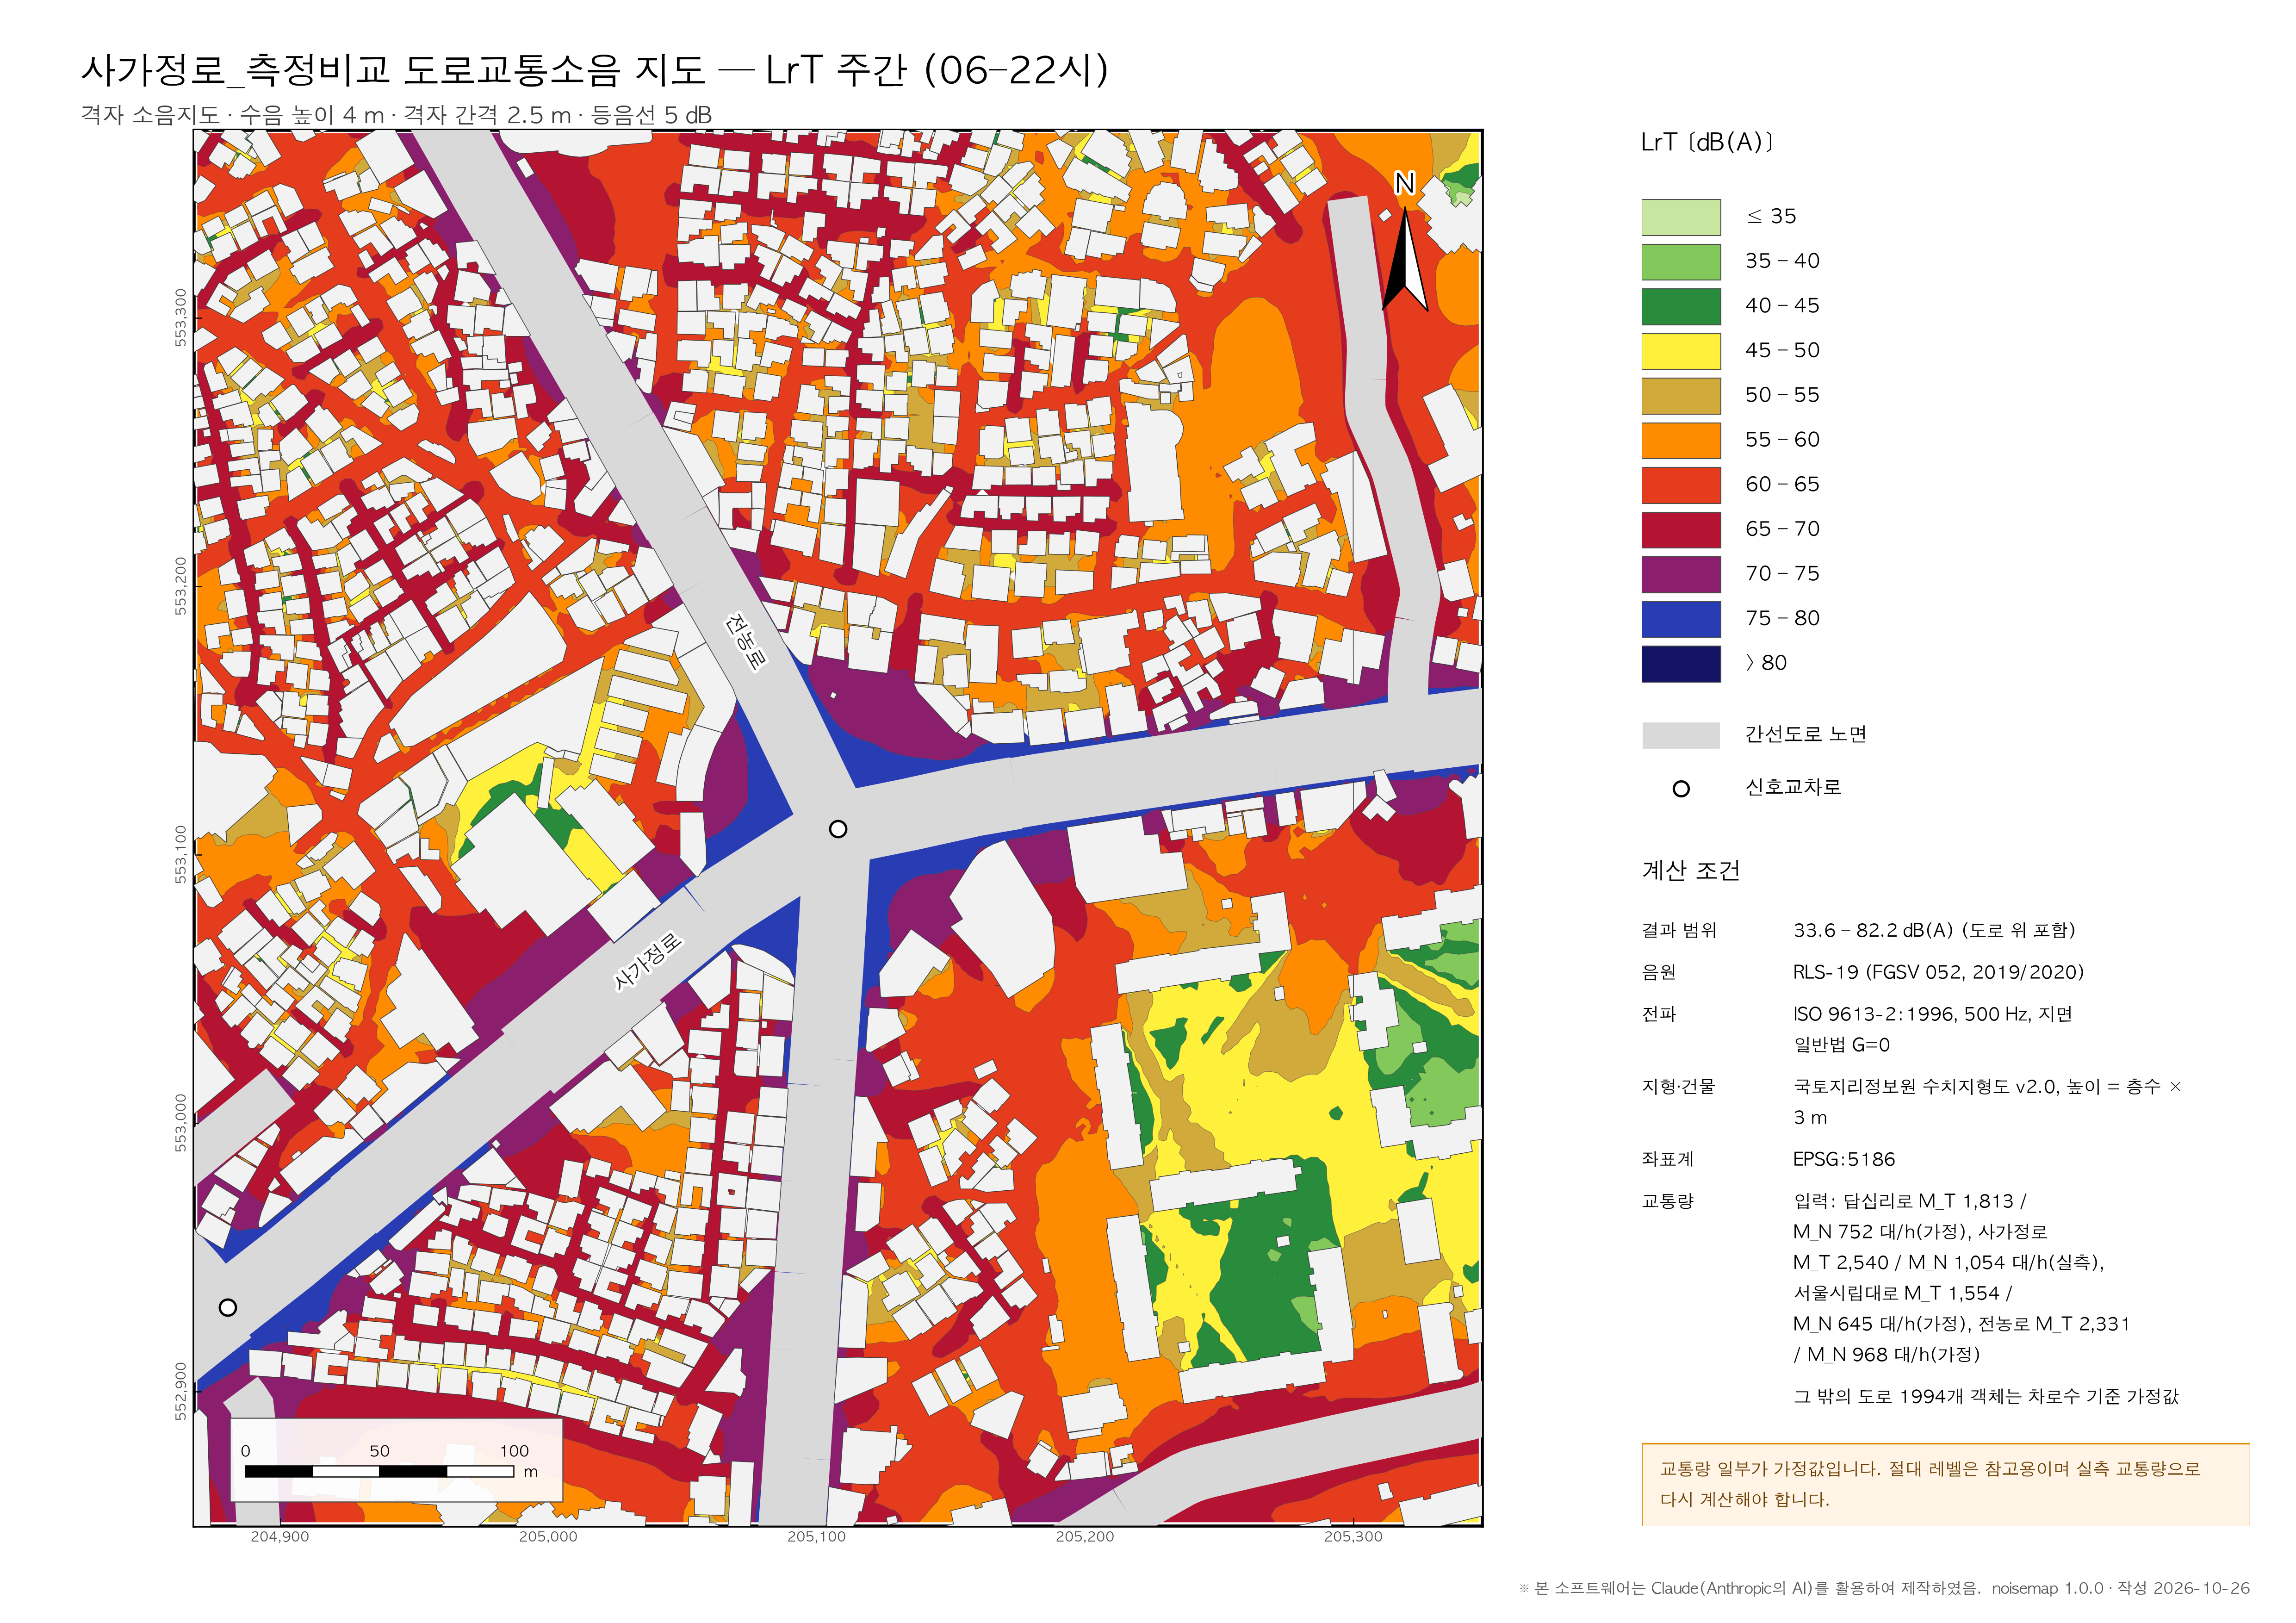
\includegraphics[width=\linewidth]{소음지도_격자_LrT_h4m_AVG.png}\par\vspace{2mm}
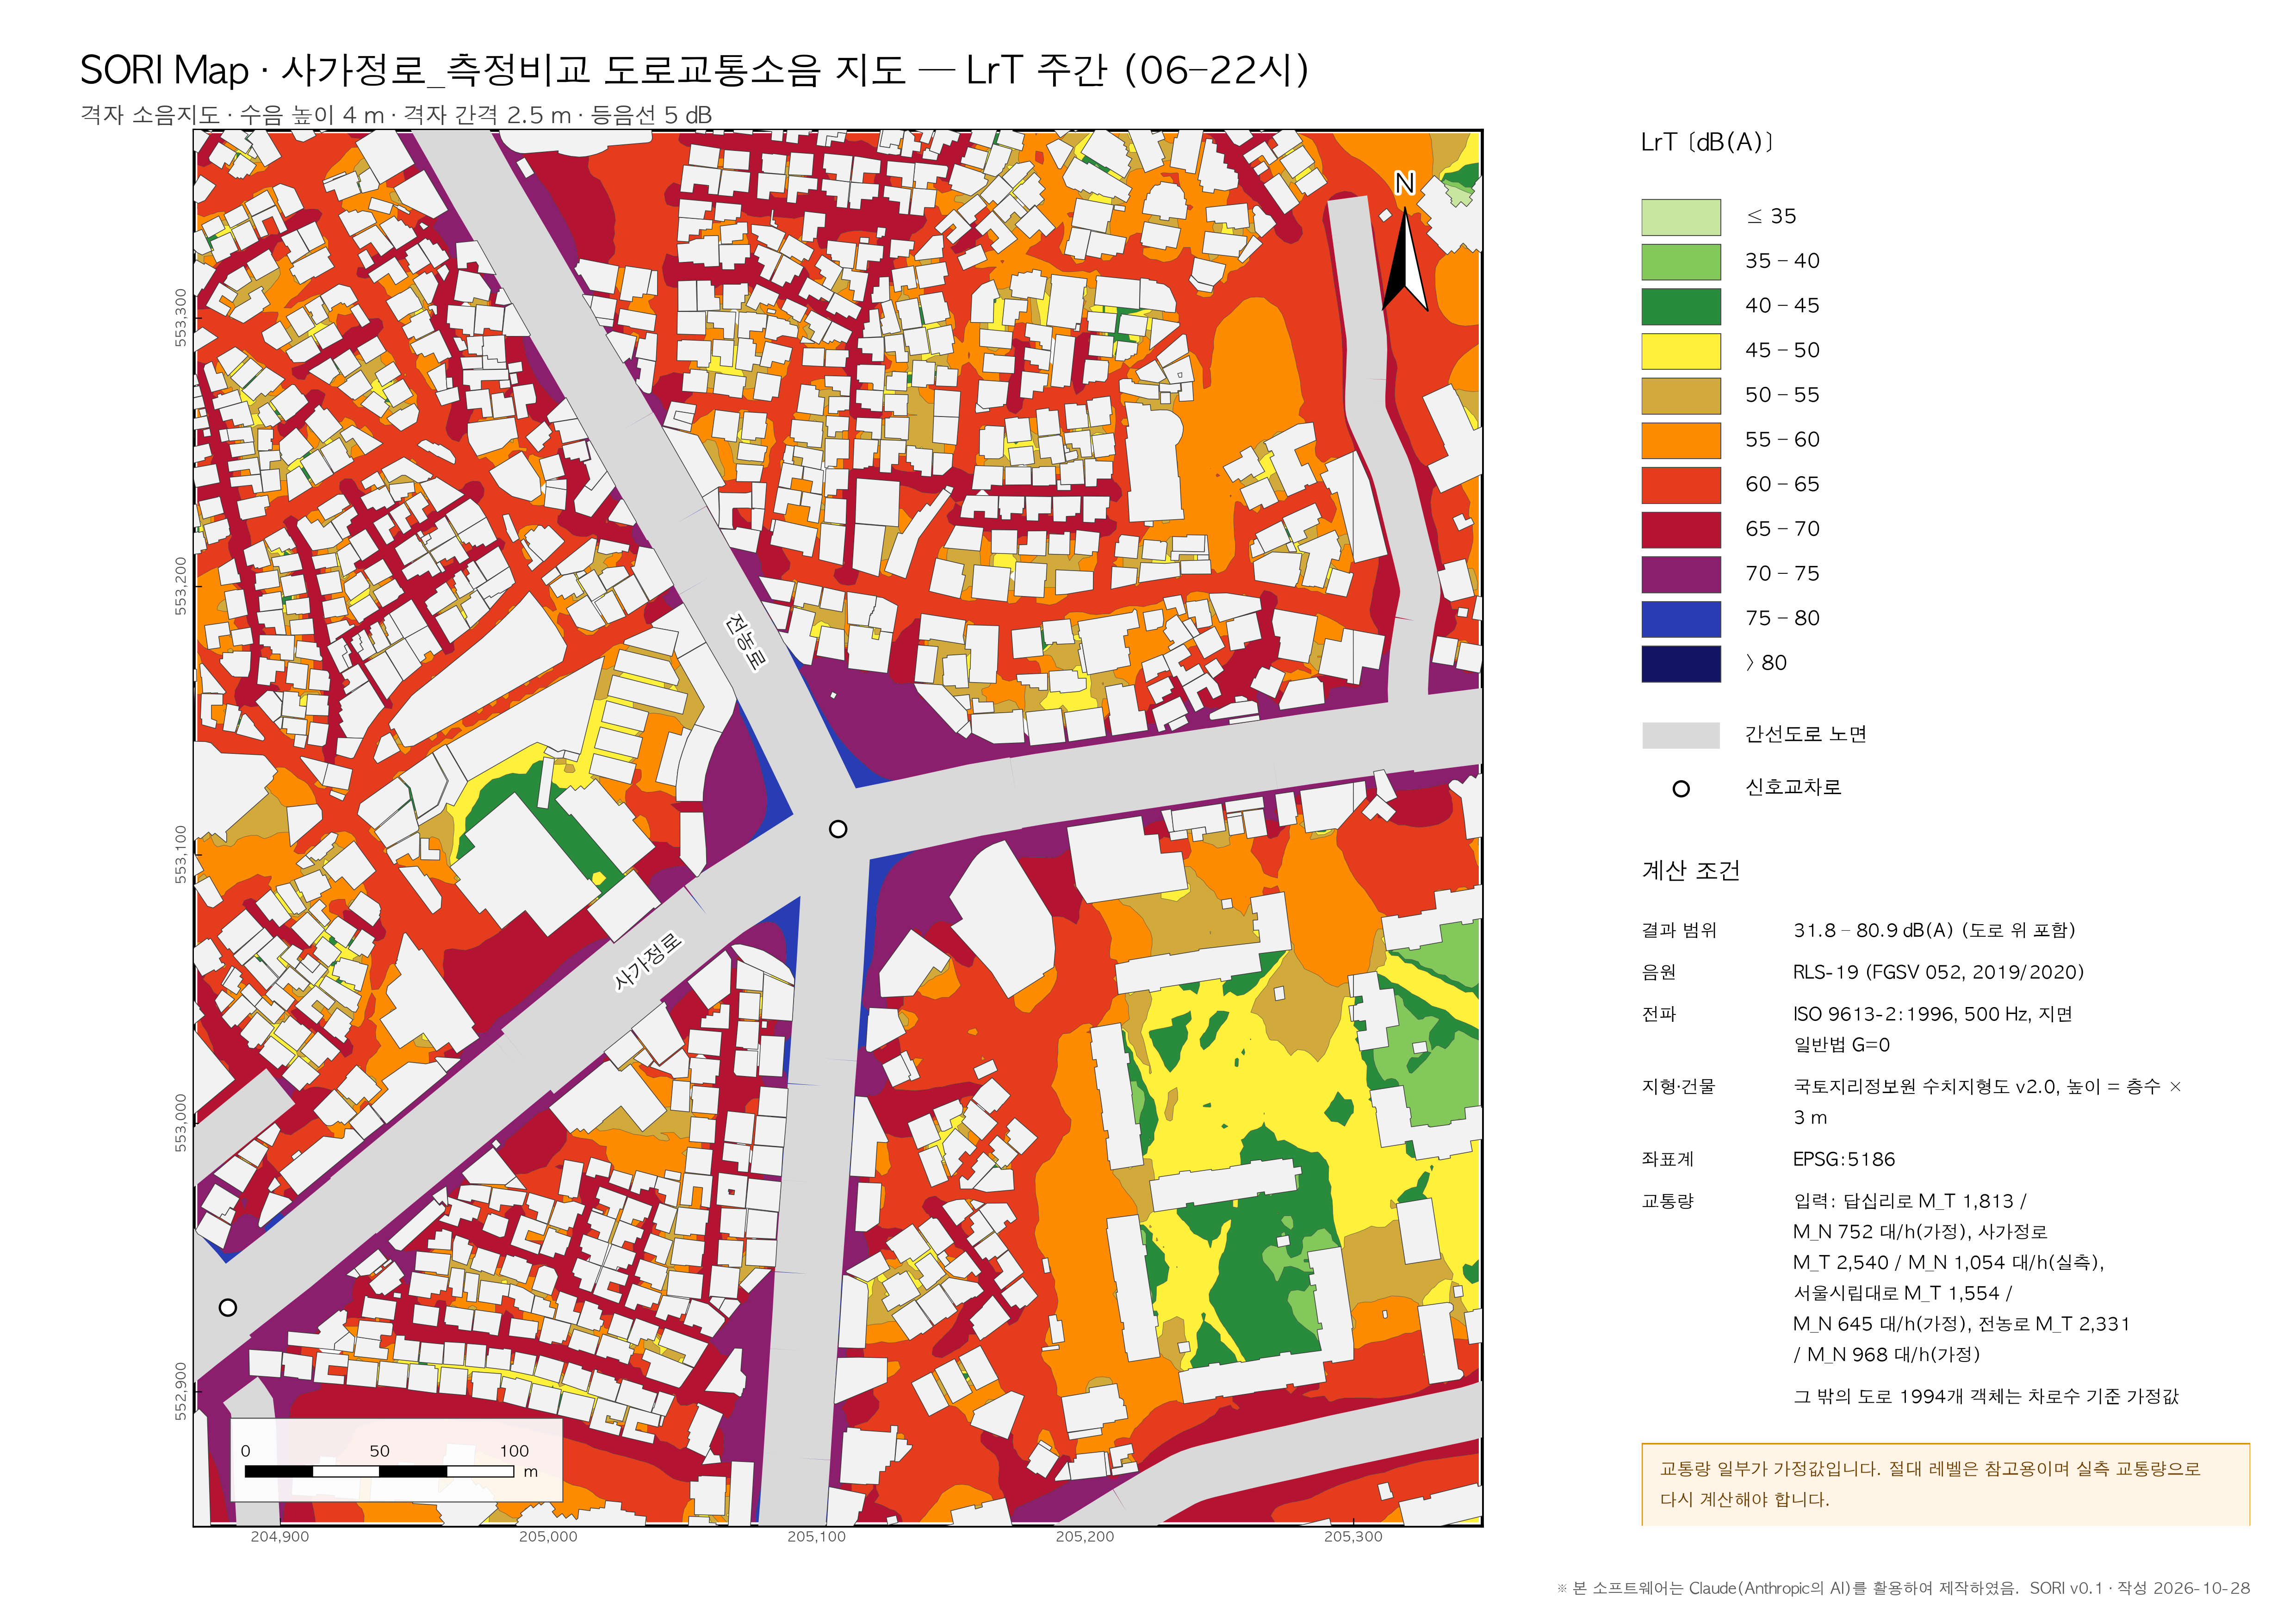
\includegraphics[width=\linewidth]{소음지도_격자_LrT_h4m_AVG_v30.png}
\caption{격자 소음지도($L_{rT}$, 높이 4 m). 위: 사가정로 50 km/h, 아래: 30 km/h}
\end{figure}

\begin{figure}[H]
\centering
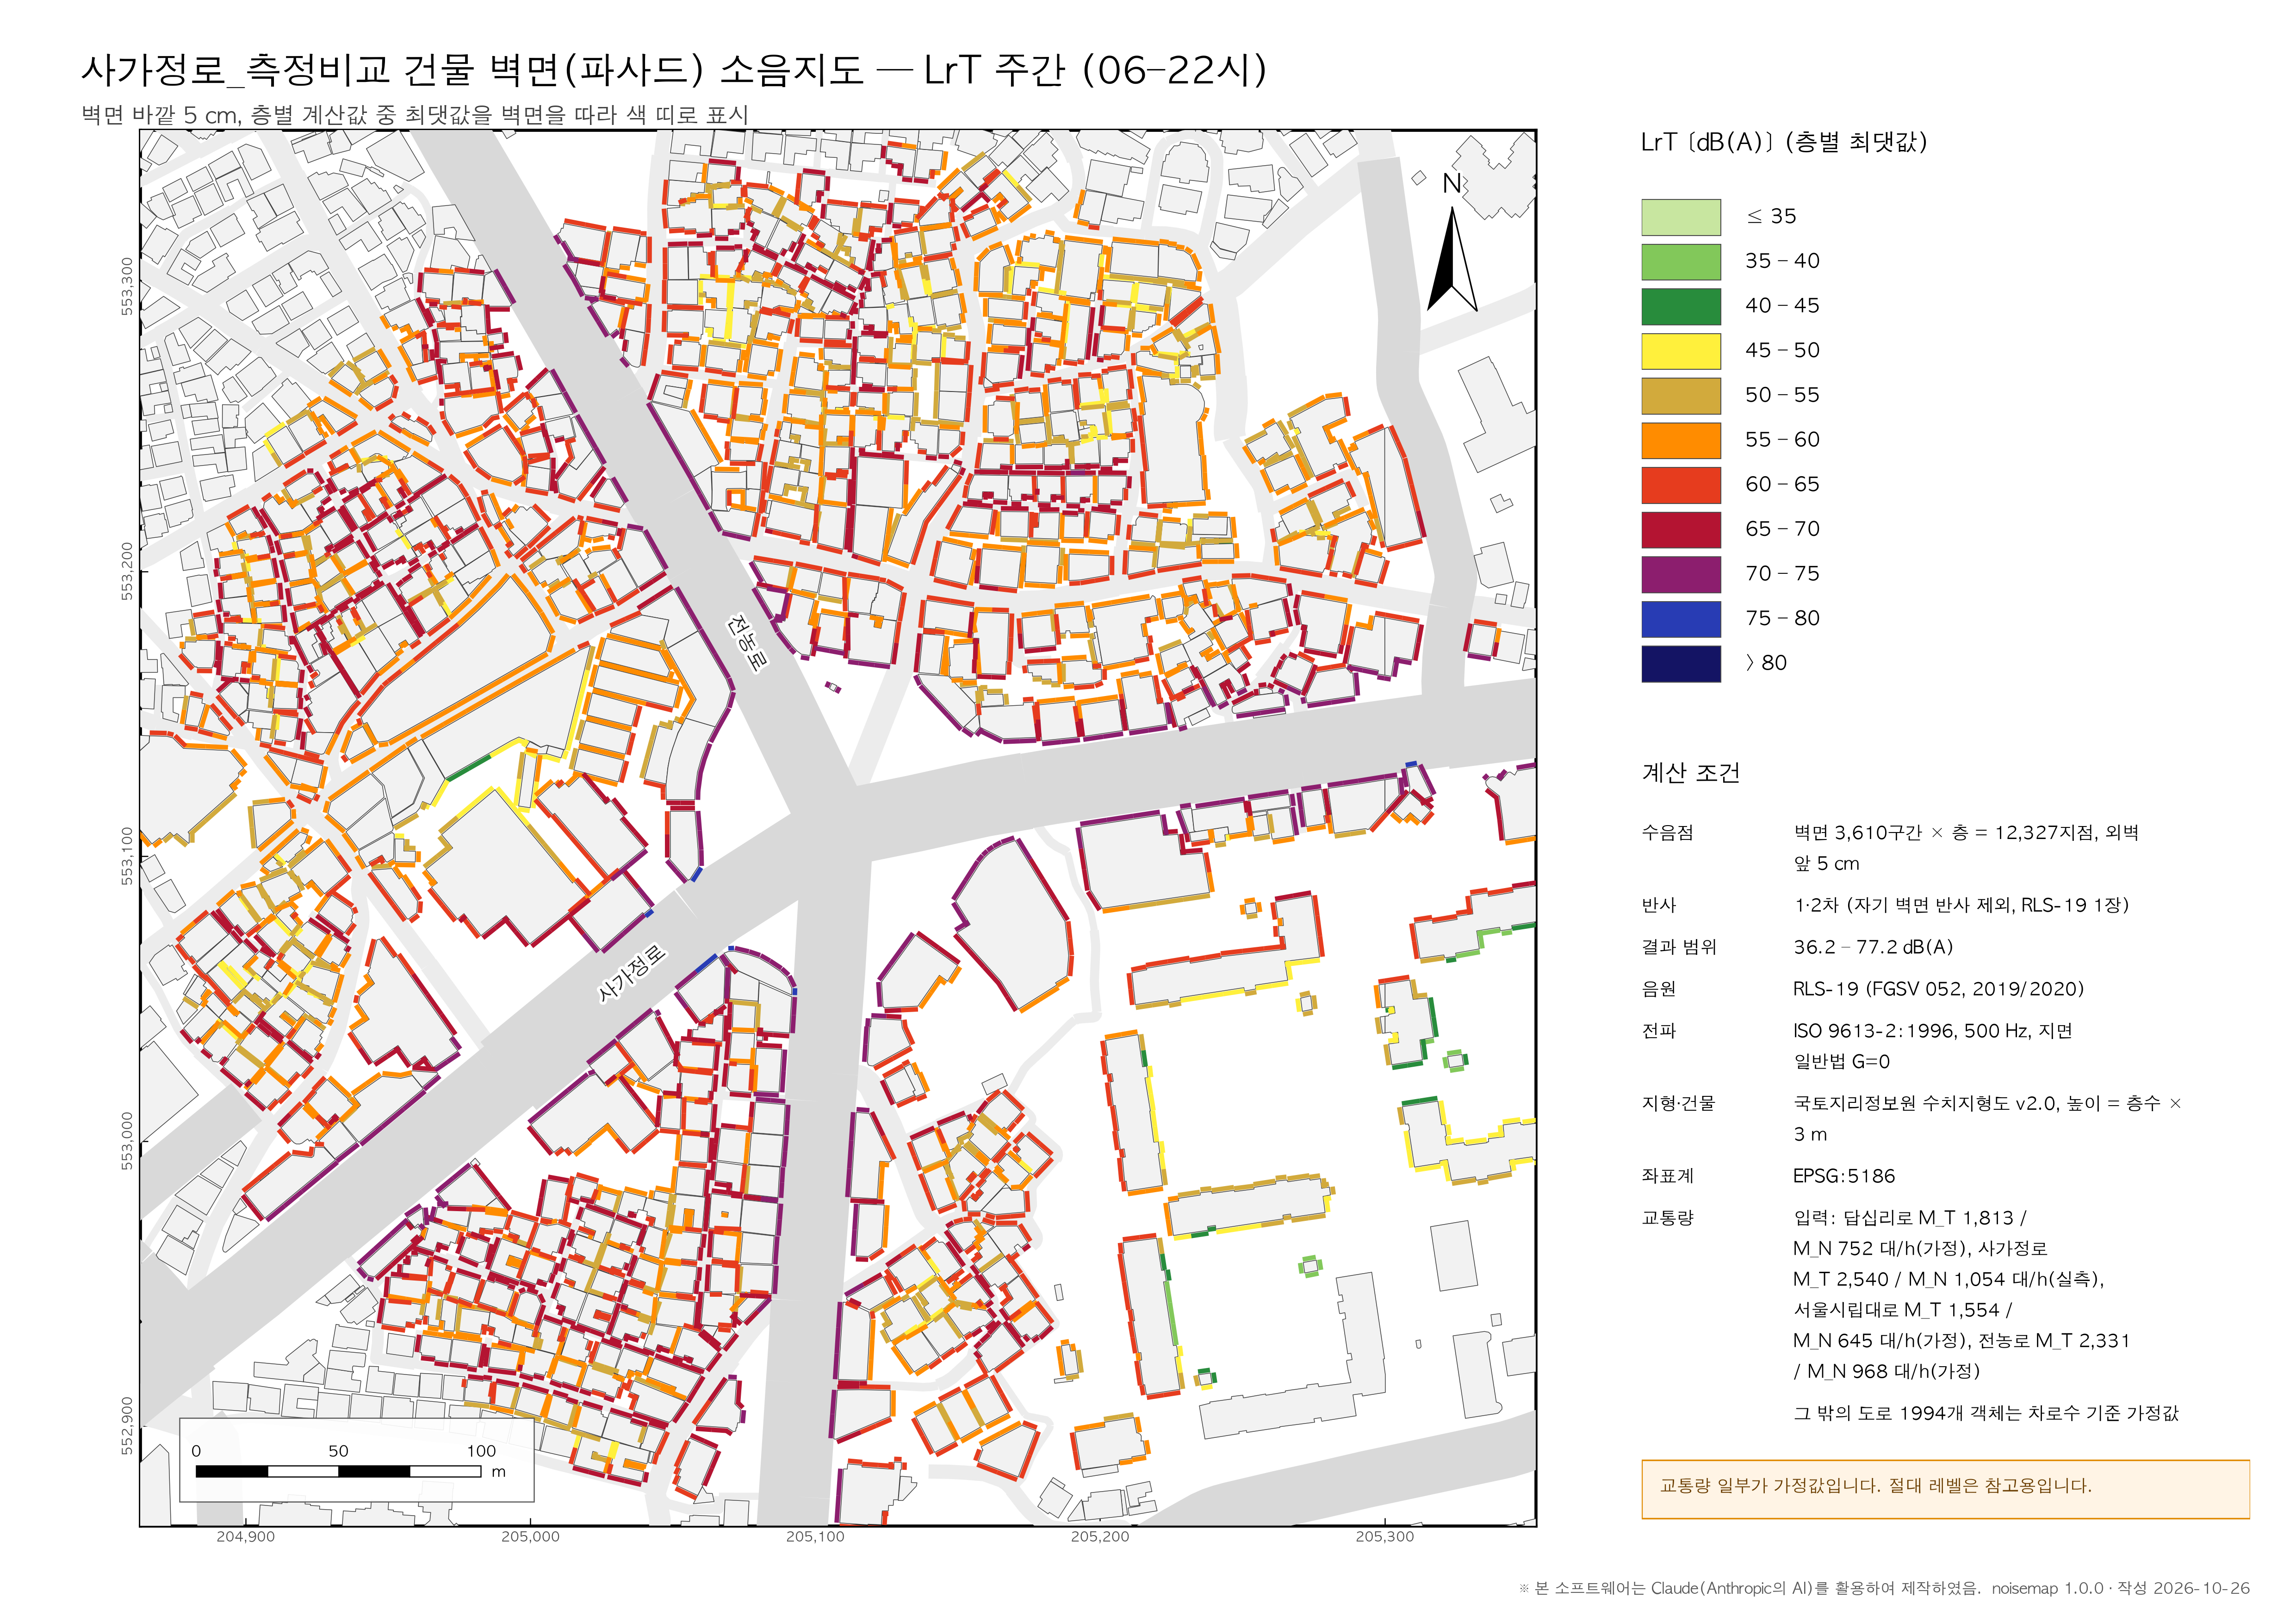
\includegraphics[width=\linewidth]{소음지도_벽면_LrT_AVG.png}\par\vspace{2mm}
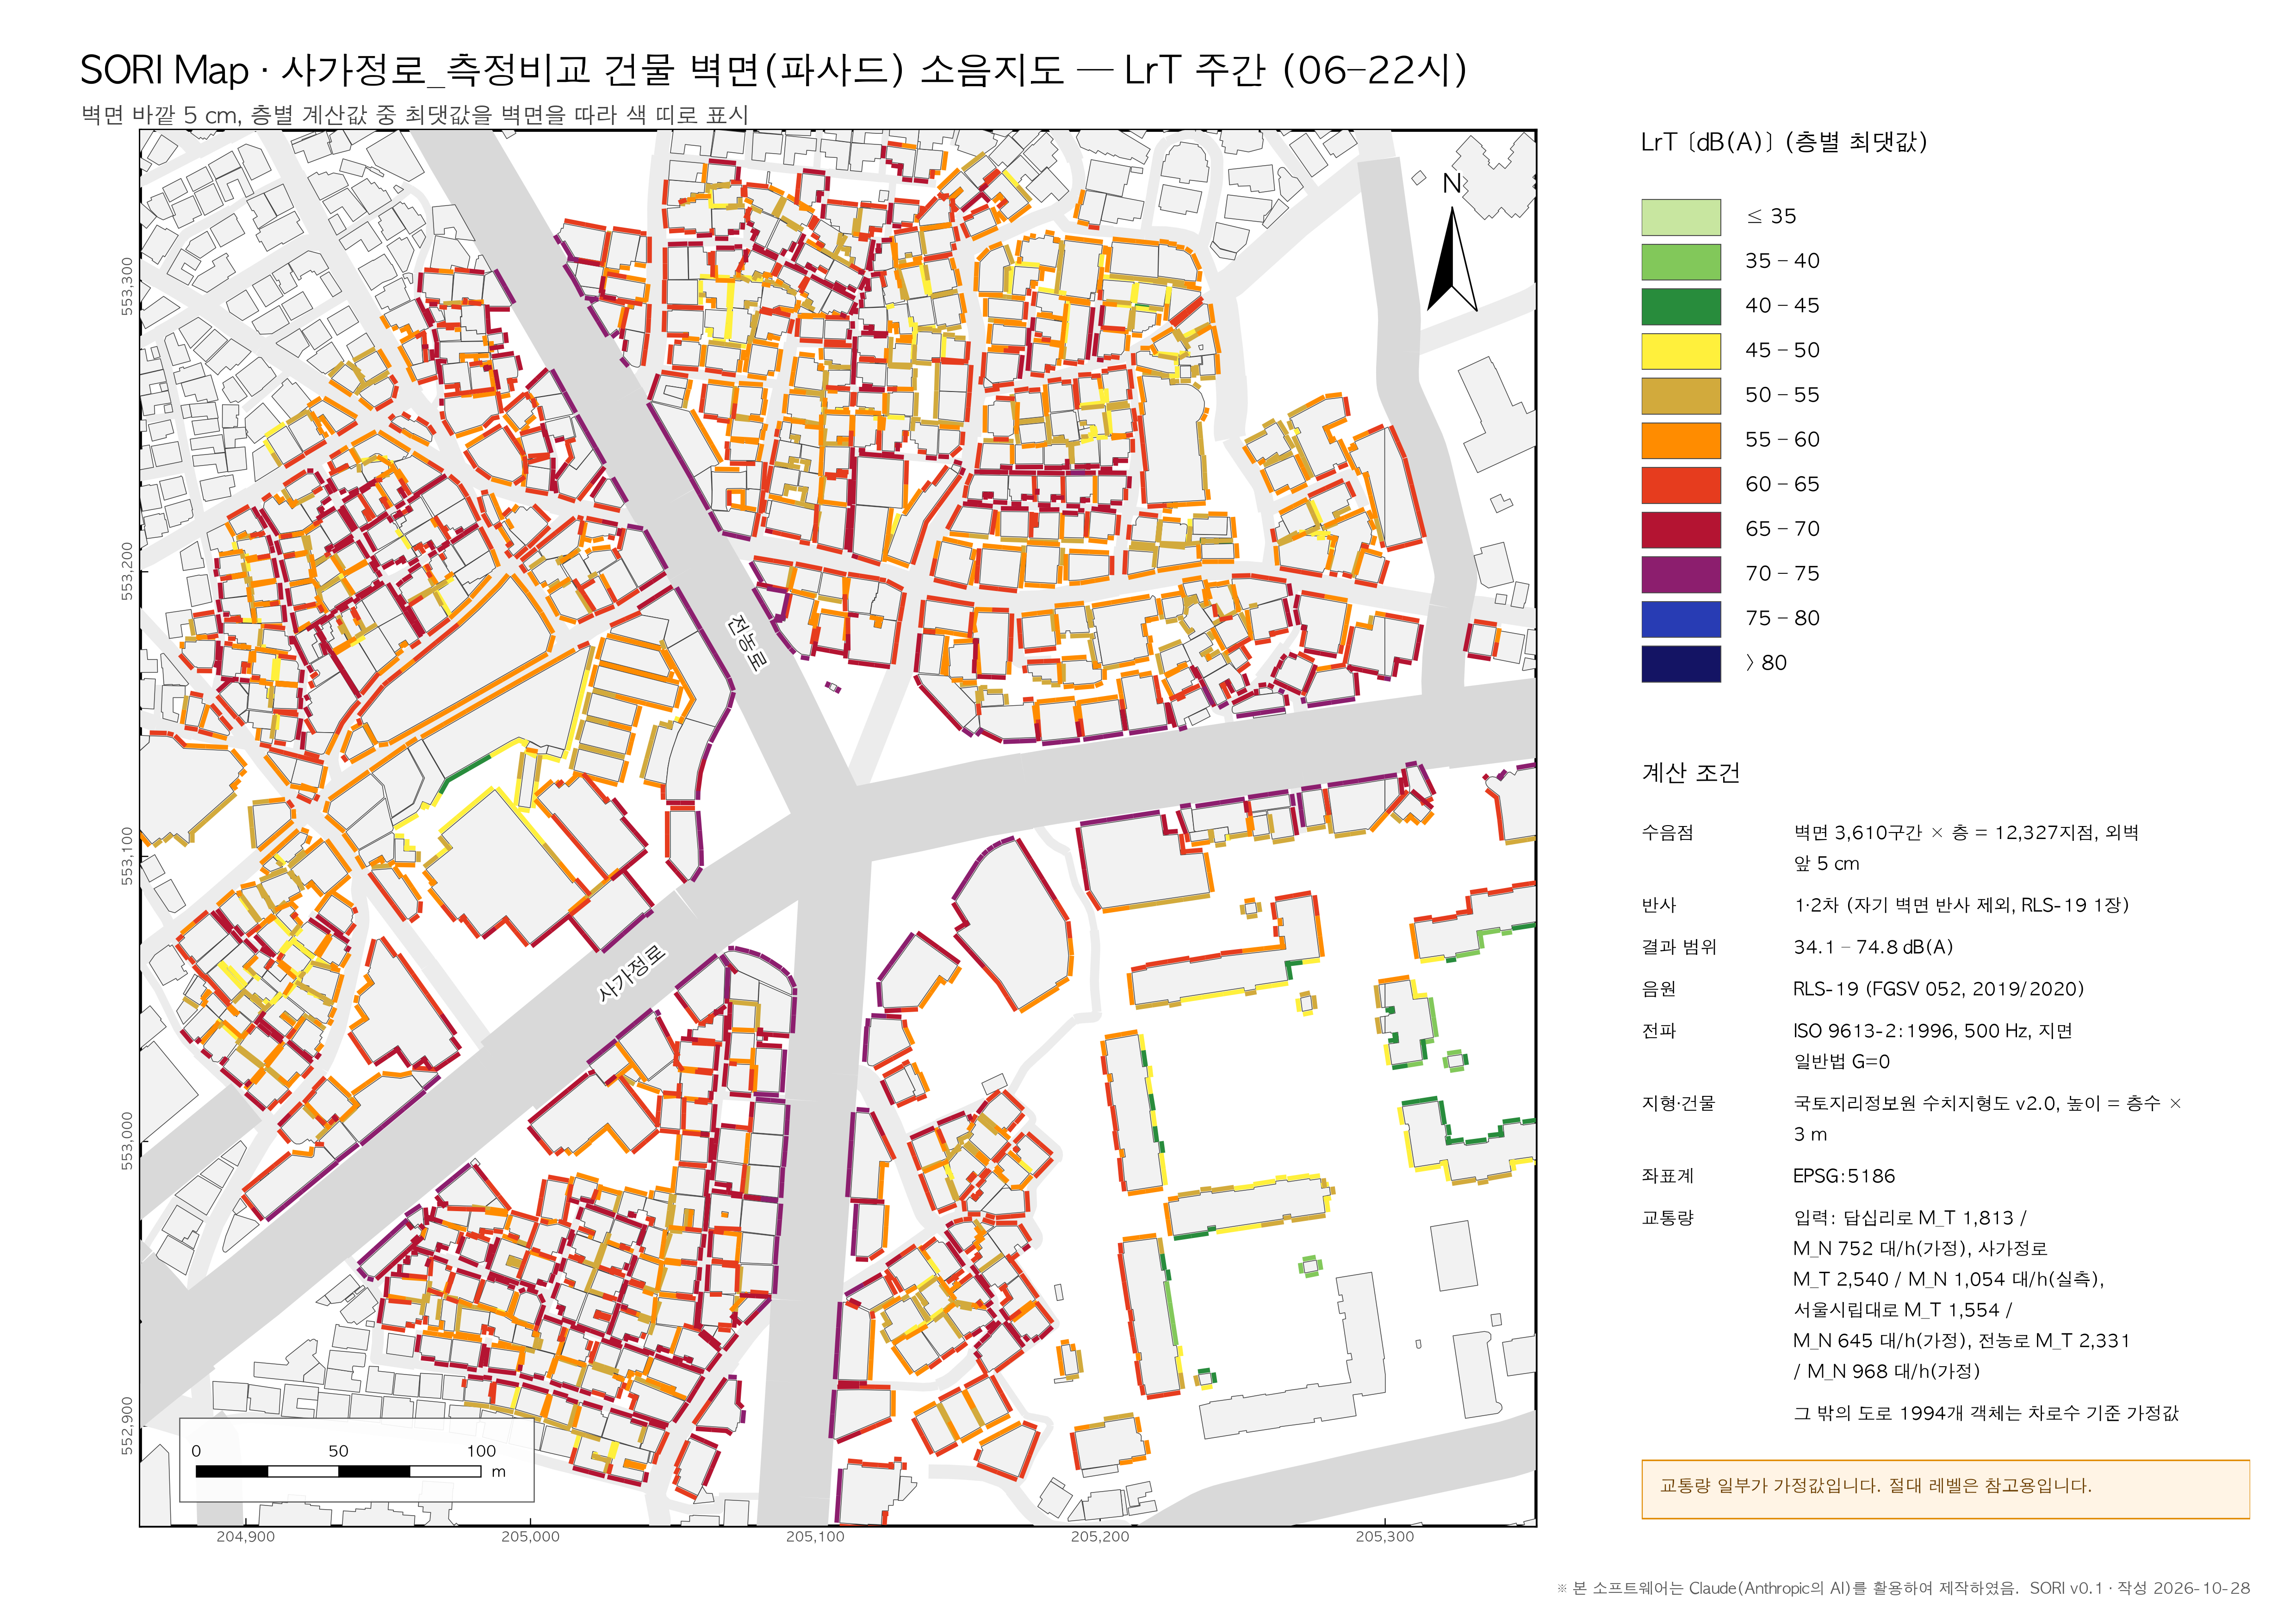
\includegraphics[width=\linewidth]{소음지도_벽면_LrT_AVG_v30.png}
\caption{건물 벽면(파사드) 소음지도($L_{rT}$, 층별 계산값 중 최댓값). 위: 사가정로 50 km/h, 아래: 30 km/h}
\end{figure}

\begin{figure}[H]
\centering
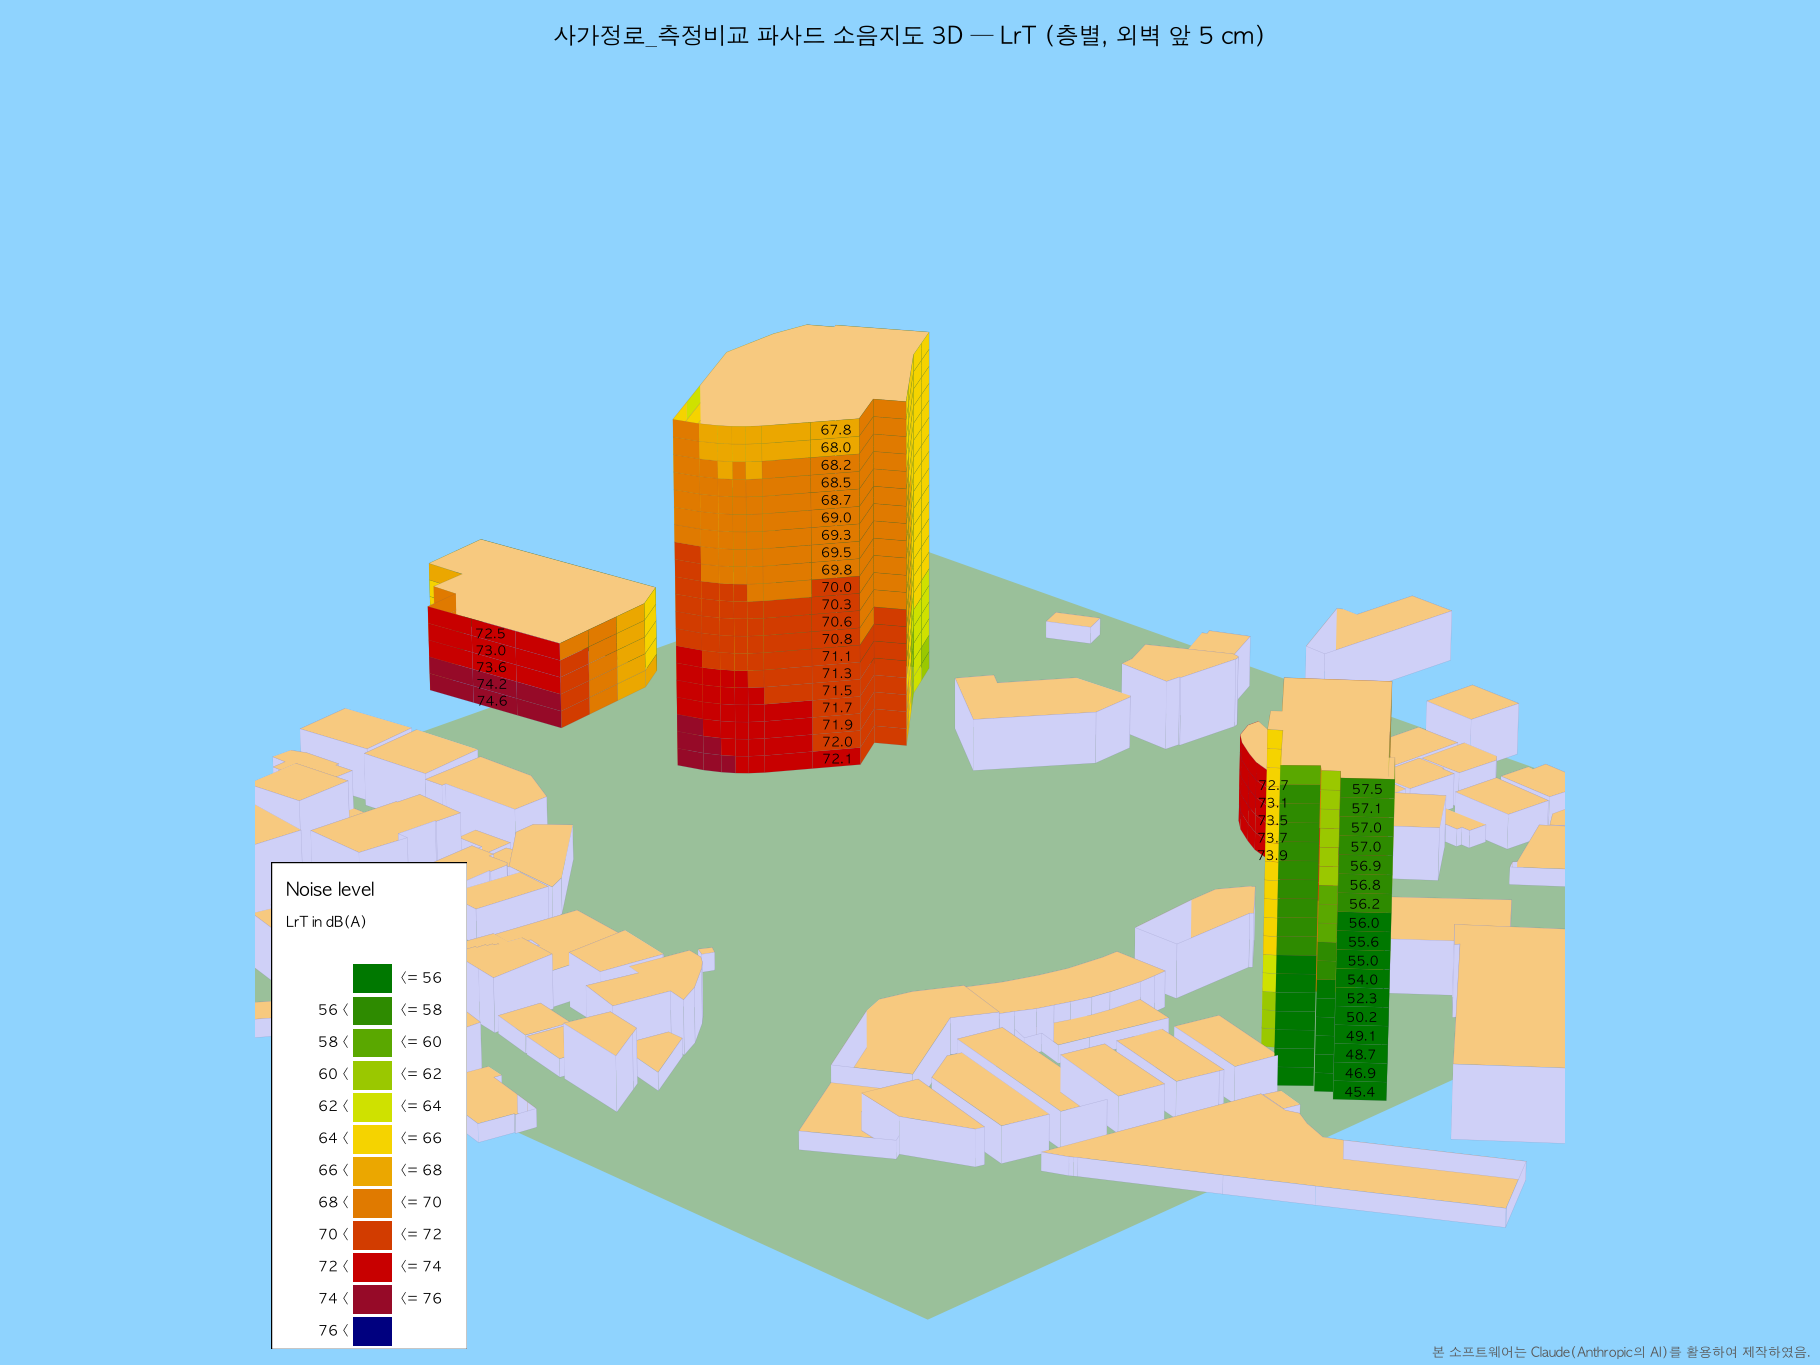
\includegraphics[width=0.49\linewidth]{소음지도_벽면3D_LrT_AVG.png}\hfill
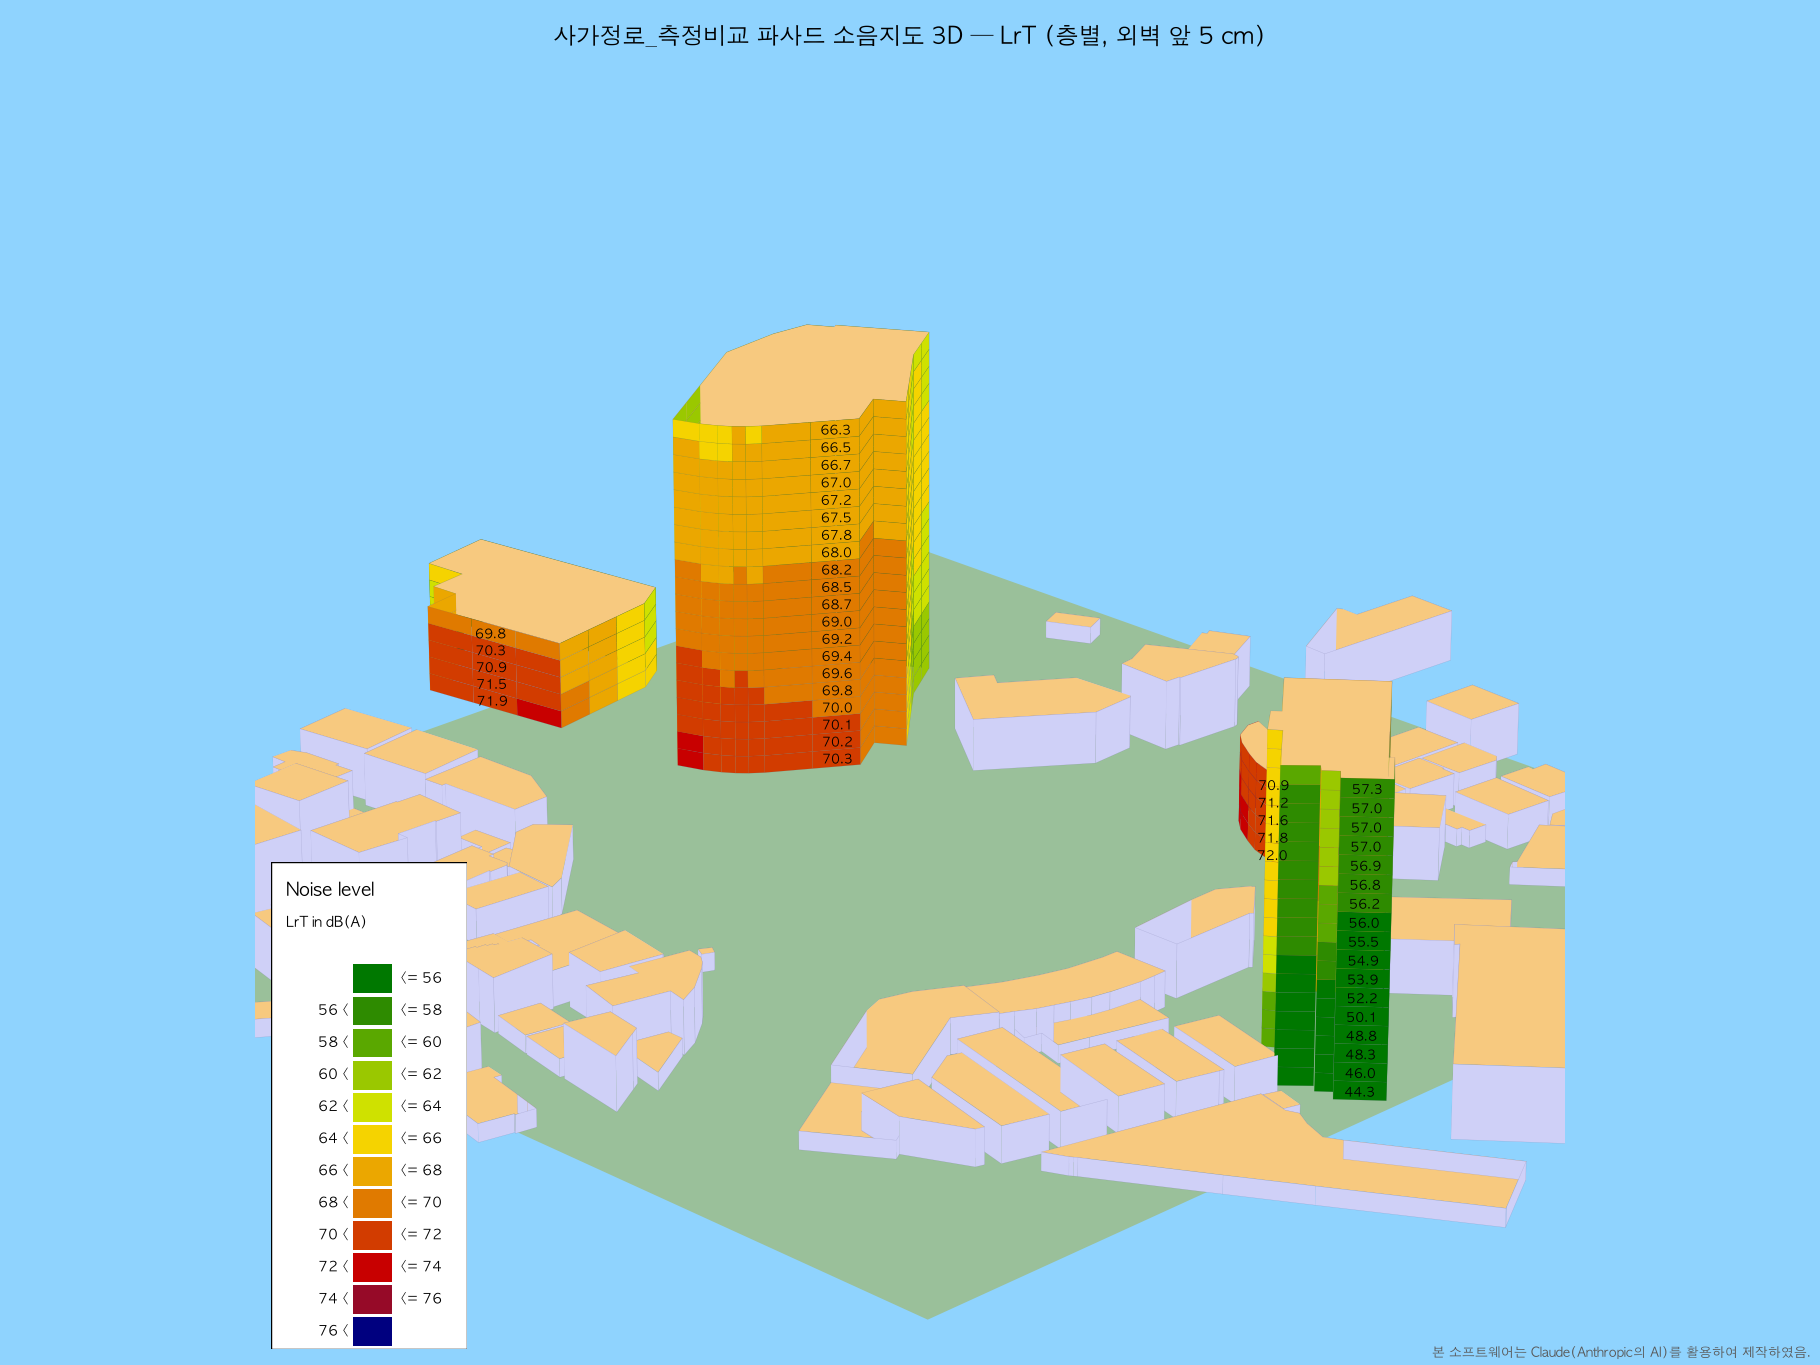
\includegraphics[width=0.49\linewidth]{소음지도_벽면3D_LrT_AVG_v30.png}\par\vspace{2mm}
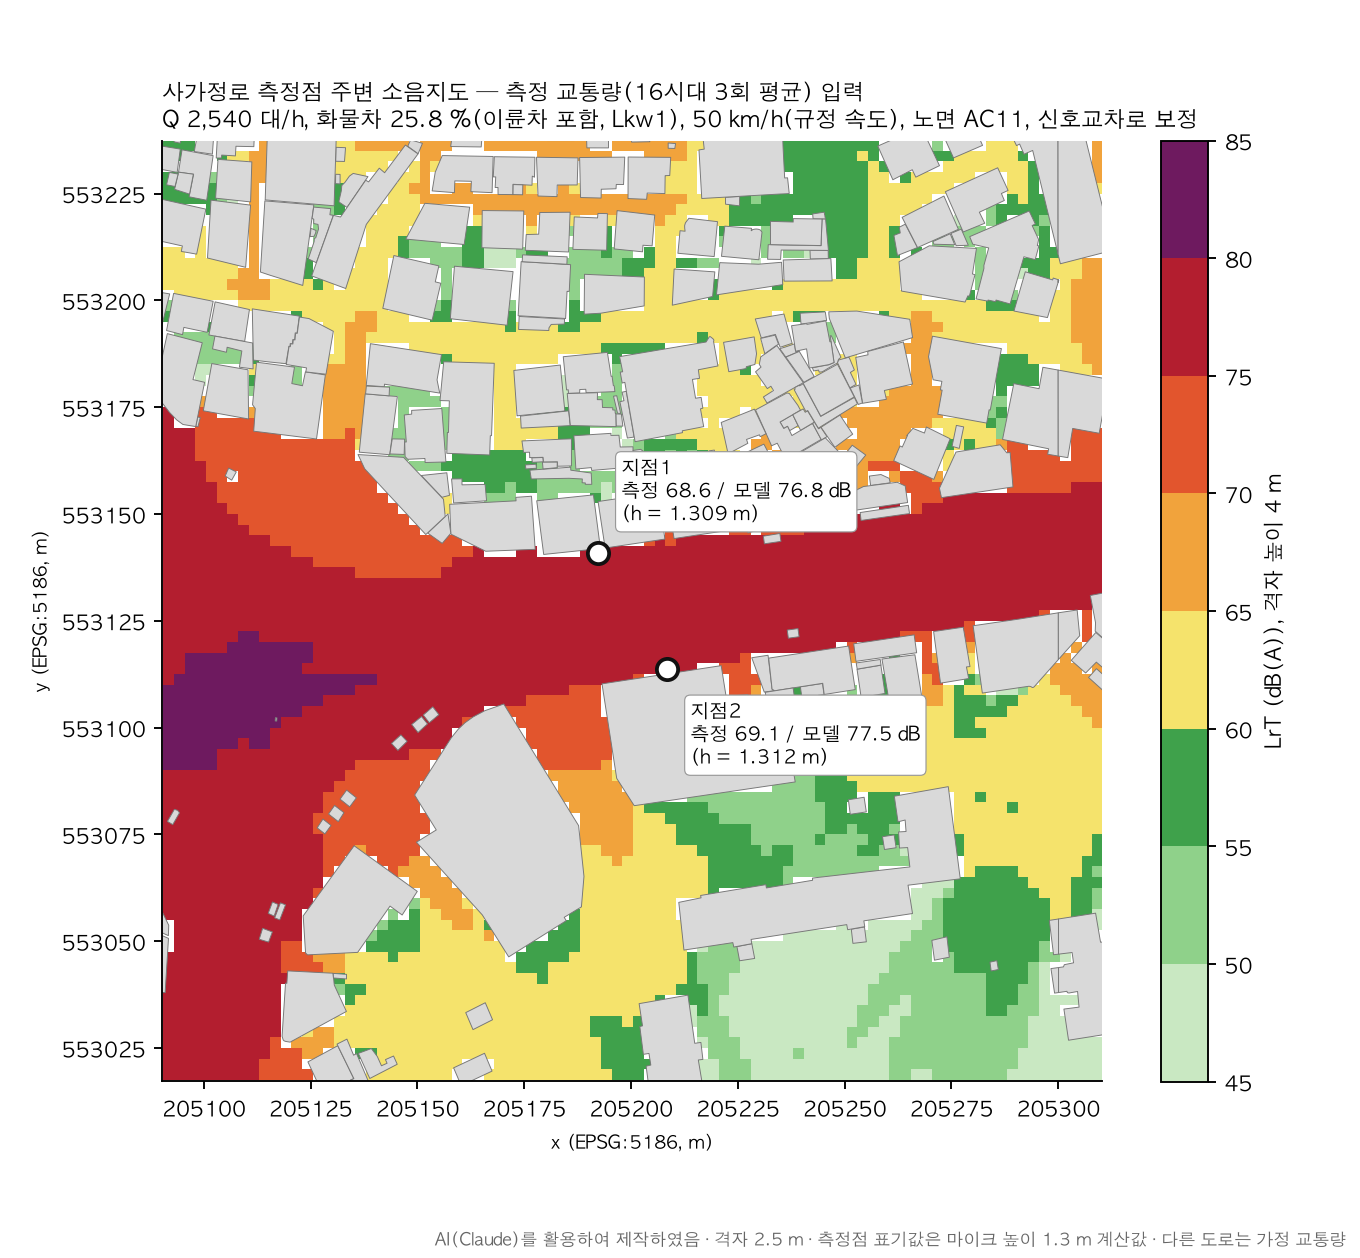
\includegraphics[width=0.49\linewidth]{소음지도_측정점주변_AVG.png}\hfill
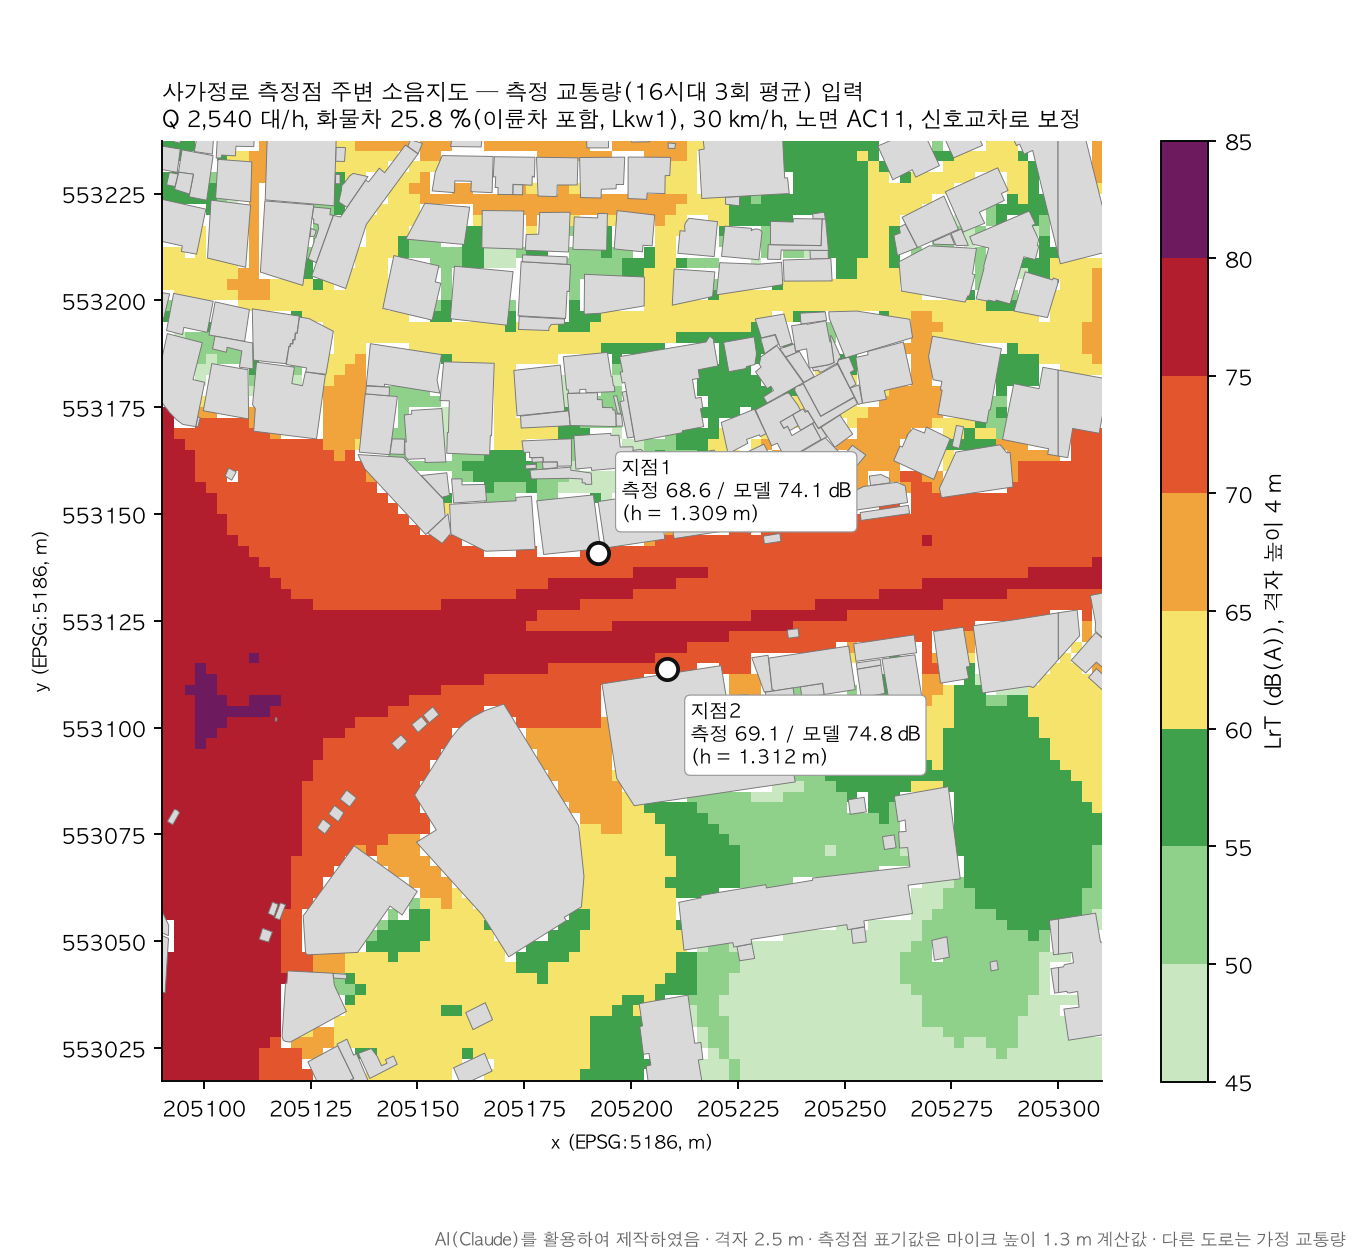
\includegraphics[width=0.49\linewidth]{소음지도_측정점주변_AVG_v30.png}
\caption{위: 측정점 주변 건물 벽면 층별 $L_{rT}$ 3D(외벽 앞 5 cm). 아래: 측정점 주변 확대 소음지도(높이 4 m). 왼쪽: 50 km/h, 오른쪽: 30 km/h. 브라우저 3D 뷰어는 model/AVG\_v50(v30)/output/noise3d.html이다}
\end{figure}

\section{불확실성 및 한계}
\footnotesize
\begin{longtable}{L{0.17}L{0.83}}
\toprule
\hd{항목} & \hd{내용} \\ \midrule
\endhead
\bottomrule
\endlastfoot
측정기 & 클래스 1 소음계 2대(RION NL-62)를 썼다. 지점2의 교정 전후 차이는 0.3 dB(93.7 → 94.0)이고, 지점1 교정 수치는 미기록이다. 두 기기는 저장 간격(100 ms와 1 s)과 밴드 가중(A와 Z)이 달랐다. 그래서 지점2는 $L_{\mathrm{Amax}}$를 다시 계산할 수 없고, 스펙트럼도 바로 비교할 수 없다. 두 기기 시계는 약 1.6 s 차이 난다(사이렌 녹음 기준, 보정하지 않음) \\ \midrule
측정 지점 수 & 사가정로 양쪽 2지점뿐이다. 전농로를 포함한 다른 접근로는 측정·계수하지 않았다. 그래서 고시의 `도로당 한 지점 이상'과 `교통소음한도 초과 건물의 50 \% 이상 지점' 요건을 충족하지 못한다 \\ \midrule
측정 횟수·시간 & 평일 16시대에 10분씩 3회 측정했다. 하루 대표값(주간 전체)이나 야간으로 일반화할 수 없다 \\ \midrule
교통량 & 각 조가 현장에서 가까운 차로를 10분 동안 셌다. 화물차와 이륜차를 구분하지 않았고 속도는 미측정이다. 계수 오차는 확인하지 않았다(영상 기록 없음) \\ \midrule
위치·좌표 & GPS는 정확도 $\pm$9--18 m이고 좌표가 소수 셋째 자리까지만 기록됐다. 그래서 수음점은 수치지도와 현장에서 잰 거리로 정했다. 도로를 따른 위치는 $\pm$5 m 정도 불확실하다. 지점2는 수치지도와 현장 거리가 1.8 m 어긋난다 \\ \midrule
기상 & 기상값은 약 8 km 떨어진 기상청 서울 관측소의 매시 관측값이고, 현장 실측이 아니다. 16시와 17시 사이 풍향이 남에서 서로 바뀌었고, 현장의 풍향·풍속은 이와 다를 수 있다. 노면 상태는 관측 기록이 없어 건조로 추정했다 \\ \midrule
모델 & 다음 입력은 가정값이다: 노면(AC11), 속도, 차종 대응, 다른 도로 교통량. 차로 수와 건물 높이는 수치지도 값을 썼다. 반사는 2차까지 계산했다. RLS-19의 속도는 허용 최고속도이고, 30 km/h 미만이면 30 km/h를 쓴다(원문 2장 용어 `Geschwindigkeit'). 구현도 같은 하한을 둔다(\texttt{rls19.speed\_rule}). 따라서 신호 대기와 정체는 속도로 표현할 수 없다. 이번 30·40 km/h 시나리오는 허용 최고속도 정의에서 벗어난 민감도 계산이다 \\ \midrule
소음지도 & 지도 값은 A가중 등가소음도로 기준과 같은 지표다. 그러나 다음 조건이 실측 \Laeq 와 다르다. (1) 교차로 보정 $D_K$가 더해진다(측정점 +0.5--0.7 dB, 교차로 가까이 최대 +2.6 dB). (2) 전파는 순풍 조건이고 장기 기상 보정 $C_{\mathrm{met}}$을 빼지 않았다. 도로변 가까이는 영향이 거의 없고, 멀어질수록 실제 평균보다 높다. (3) 격자는 높이 4 m, 벽면은 외벽 앞 5 cm에서 그 벽 자신의 반사를 뺀 값이라, 측정(높이 1.3 m, 벽 앞 1.0--1.1 m, 벽 반사 포함)과 위치 조건이 다르다. (4) 이 구간에서 측정보다 5--8 dB 높게 계산되므로 초과 면적·건물 수는 과대 추정일 수 있다. (5) 초과 판정선은 관리기준 가목 주간 68 dB(A) 하나로, 용도지역별 기준(지점1 쪽 나목 73 등)을 나눠 적용하지 않았다. (6) 야간 지도는 야간 교통량이 측정되지 않아 쓰지 않았다 \\
\end{longtable}
\addtocounter{table}{-1}
\normalsize

%% ------------------------------------------------------------------
\section{결론 및 소음지도 작업에 대한 시사점}
\subsection{결론}
\begin{enumerate}
\item 전농사거리 동쪽 사가정로 도로변(교차로에서 약 90--100 m)의 평일 16시대 \Laeq 는 지점1 68.5 dB(A), 지점2 69.1 dB(A)다(산술평균). 정수로는 두 지점 모두 69 dB(A)다.
\item 제3종일반주거지역인 도로 남측(지점2)은 환경기준(도로변 65)을 4 dB, 도로 관리기준(가목 68)을 1 dB 넘는다. 근린상업지역인 도로 북측(지점1)은 두 기준 모두 이하다. 측정 횟수·간격 요건을 채우지 못해 \textbf{참고 평가}에 그친다. 밤 시간대는 \textbf{평가 불가}다.
\item 측정 교통량과 규정 속도를 넣은 소음지도 모델은 측정값보다 평균 8.3 dB 높게 계산했다. 이는 고시 검증 기준(평균 $\pm$3 dB)을 충족하지 못한다. 다만 회차 간 표준편차(0.65 dB)와 두 지점 사이의 상대 차이는 측정과 잘 맞는다. 따라서 차이는 모델 전체에 걸친 일정한 치우침으로 본다. 직접음 계산은 구현한 식과 일치한다(손계산과 0.2 dB 이내). 원문 수치표와 공식 시험과제(TEST-20)와의 대조는 하지 않았다.
\item 조합 96개를 실제로 실행했다(표 \ref{tab:combo}). 기본 조건(50 km/h, AC11)에서 속도 30 km/h와 화물차 절반 Pkw를 함께 가정하면 차이가 $-$8.2/$-$8.5에서 $-$4.3/$-$4.4 dB로 3.9--4.0 dB 줄어든다(지점1/지점2). $D_K$·$D_{\mathrm{refl}}$을 끄면 0.9--1.2 dB 더 줄고, 화물차를 전부 Pkw로 보면 $-$1.3/$-$1.5 dB까지 줄어 고시 기준(평균 $\pm$3 dB) 안에 든다. 다만 이 마지막 조합은 차종 가정이 극단적이고, 30 km/h는 RLS-19의 속도 정의(허용 최고속도)를 벗어난 값이다. 지면 감쇠를 RLS-19식으로 처리하면 측정점이 1.5--1.9 dB 더 낮아진다(표 \ref{tab:ground}, 조합과 별도 계산). 어느 가정이 실제에 맞는지는 이번 측정 자료로 가릴 수 없다.
\item 같은 교통량으로 그린 주간 소음지도(6.8절)에서 사가정로 속도를 50에서 30 km/h로 낮추면 사가정로 변 벽면이 2.6--2.9 dB 낮아진다. 68 dB(A) 초과 벽면·층은 9.9 \%에서 7.5 \%로, 격자 초과 비율은 34.4 \%에서 33.0 \%로 준다. 다른 도로의 가정 교통량은 그대로이므로 지역 전체의 초과 범위는 크게 줄지 않는다. 이 지도는 측정보다 5--8 dB 높게 계산되는 조건이라 초과 범위는 참고값이다.
\end{enumerate}

\subsection{소음지도 작업에 대한 시사점}
\small
\begin{longtable}{L{0.22}L{0.78}}
\toprule
\hd{구분} & \hd{내용} \\ \midrule
\endhead
\bottomrule
\endlastfoot
입력 자료 보완 & 사가정로 주행속도를 실측한다(스피드건 또는 영상). 노면 종류와 포장 이력을 확인한다. 차량은 RLS-19 차종(Pkw, Lkw1 3.5 t 초과, Lkw2, 이륜차 별도)에 맞춰 나눠 센다. 측정점 주변 학교·병원·어린이집 등의 부지경계 50 m 이내 여부를 확인한다 \\ \midrule
모델 설정 조정 검토 & 노면 매핑(아스팔트 → AC11)을 소음지도 기본 설정에 넣을지 검토한다. 신호교차로 보정 옵션(dk\_rule: nearest\_signal)은 원문 3.3.7의 기준 교차점 정의와 달라, 기본 설정으로 삼지 않는 쪽이 원문에 맞다. 지면 감쇠를 ISO 일반법($G = 0$)으로 둘지 RLS-19식(대안법)으로 둘지도 검토한다(표 \ref{tab:ground}). 신호 교차로 접근부의 속도를 규정 속도보다 낮게 줄지도 검토한다. 그 전까지 소음지도의 절대값은 이 구간에서 5--8 dB 높게 나올 수 있음을 함께 표시한다 \\ \midrule
추가 측정 필요 & 공정시험기준의 횟수·간격(낮 4회, 2--4시간 간격, 야간 포함)을 지켜 다시 측정한다. 전농로 등 다른 접근로에도 측정점을 둔다. 두 소음계의 설정(저장 간격, 밴드 가중)을 같게 맞춘다. 교정 수치는 양쪽 모두 기록한다 \\
\end{longtable}
\addtocounter{table}{-1}
\normalsize

%% ------------------------------------------------------------------
\clearpage\section*{부록 A. 원자료 목록}\addcontentsline{toc}{section}{부록 A. 원자료 목록}
\footnotesize
\begin{longtable}{L{0.30}L{0.24}L{0.14}L{0.32}}
\toprule
\hd{파일} & \hd{종류} & \hd{지점·회차} & \hd{비고} \\ \midrule
\endhead
\bottomrule
\endlastfoot
Auto\_0306, 0307, 0308 & NL-62 Auto Store(설정 .rnh, AUTO\_LEQ, AUTO\_LP, SOUND .wav) & 지점1 · 1--3회 & 폴더명 `하행\_임양록'(지도 기준으로는 상행 쪽) \\ \midrule
Auto\_0303, 0304, 0305 & 같음 & 지점2 · 1--3회 & 폴더명 `상행\_임영택'(지도 기준으로는 하행 쪽) \\ \midrule
야장 사진 4장, 측정 기록표 & 현장 기록 & 지점1·2 & 교통량, 교정, 이벤트 시각 \\ \midrule
SHA256SUMS\_원본.txt & 원본 해시(34개 파일) & --- & 분석은 복사본(raw\_copy)으로 했다 \\ \midrule
results/*.csv, figures/*.png & 분석 결과 & --- & field\_measurement/2026-10-22 \\ \midrule
model/AVG\_v50, AVG\_v30/output/ & 소음지도 계산 원자료(grid\_result.csv, facade\_result.csv, noise3d.html, 야간 지도) & --- & git 무시 대상. scripts/model\_compare.py로 다시 만든다(\ref{sec:map}절) \\
\end{longtable}
\addtocounter{table}{-1}
\normalsize
{\small 원본 보관 위치: 측정자료 원본 폴더(\texttt{[소음진동설계]\_261022\_측정자료}). 원본은 수정하지 않았다.\par}

\section*{부록 B. 교정 기록}\addcontentsline{toc}{section}{부록 B. 교정 기록}
\small
\begin{longtable}{C{0.12}C{0.11}C{0.14}C{0.14}C{0.12}C{0.37}}
\toprule
\hd{회차} & \hd{장비} & \hd{측정 전} & \hd{측정 후} & \hd{차이} & \hd{판정} \\ \midrule
\endhead
\bottomrule
\endlastfoot
1--3회 전체 & SLM-1 & 미기록 & 미기록 & --- & 교정은 했지만(사용자 확인) 수치가 없어 편차는 미확인 \\ \midrule
1--3회 전체 & SLM-2 & 93.7 dB & 94.0 dB & 0.3 dB & 교정기 94 dB, 1 kHz 기준. 회차별 점검 기록은 없음 \\
\end{longtable}
\addtocounter{table}{-1}
\normalsize
{\small 교정 전후 허용 편차는 공정시험기준에서 규정을 찾지 못했다(미확인). 본 조사에서 따로 정하지도 않았다.\par}

\section*{부록 C. 현장 사진}\addcontentsline{toc}{section}{부록 C. 현장 사진}
측정 장비를 설치한 모습과 주변 사진은 본 보고서에 첨부하지 않았다. 원자료에는 야장 사진만 있다.

\section*{부록 D. 교통량 원자료}\addcontentsline{toc}{section}{부록 D. 교통량 원자료}
\small
\begin{longtable}{C{0.08}C{0.16}L{0.30}C{0.14}C{0.18}C{0.14}}
\toprule
\hd{회차} & \hd{시각} & \hd{방향(계수 조)} & \hd{승용차} & \hd{화물차(이륜차 포함)} & \hd{합계} \\ \midrule
\endhead
\bottomrule
\endlastfoot
1 & 16:15--16:25 & 상행(서행), 지점1 조 & 148 & 33 & 181 \\
1 & 16:15--16:25 & 하행(동행), 지점2 조 & 180 & 76 & 256 \\ \midrule
2 & 16:28--16:38 & 상행(서행), 지점1 조 & 138 & 54 & 192 \\
2 & 16:28--16:38 & 하행(동행), 지점2 조 & 180 & 68 & 248 \\ \midrule
3 & 16:41--16:51 & 상행(서행), 지점1 조 & 133 & 47 & 180 \\
3 & 16:41--16:51 & 하행(동행), 지점2 조 & 163 & 50 & 213 \\
\end{longtable}
\addtocounter{table}{-1}
\normalsize
{\small 단위는 대/10분이다. 지점2 조의 값은 야장의 `0--5분' 칸에 적혀 있지만 10분 계수다(사용자 확인).\par}

\section*{부록 E. 회차별 비교표}\addcontentsline{toc}{section}{부록 E. 회차별 비교표}
\footnotesize
\begin{longtable}{C{0.08}C{0.08}C{0.12}C{0.08}C{0.11}C{0.11}C{0.11}C{0.10}C{0.10}C{0.11}}
\toprule
\hd{지점} & \hd{회차} & \hd{Q (대/h)} & \hd{p (\%)} & \hd{측정 \Laeq} & \hd{$L_{\mathrm{Amax}}$} & \hd{$L_{90}$} & \hd{차이 30} & \hd{차이 40} & \hd{차이 50} \\ \midrule
\endhead
\bottomrule
\endlastfoot
1 & 1 & 2622 & 24.9 & 68.1 & 85.4 & 61.4 & $-$6.0 & $-$7.1 & $-$8.6 \\
1 & 2 & 2640 & 27.7 & 68.3 & 79.9 & 60.8 & $-$6.2 & $-$7.2 & $-$8.8 \\
1 & 3 & 2358 & 24.7 & 69.2 & 82.8 & 62.0 & $-$4.6 & $-$5.7 & $-$7.3 \\ \midrule
2 & 1 & 2622 & 24.9 & 68.9 & 81.5 & 61.4 & $-$6.0 & $-$7.1 & $-$8.7 \\
2 & 2 & 2640 & 27.7 & 69.0 & 84.9 & 60.0 & $-$6.1 & $-$7.2 & $-$8.8 \\
2 & 3 & 2358 & 24.7 & 69.3 & 85.1 & 59.4 & $-$5.0 & $-$6.1 & $-$7.7 \\
\end{longtable}
\addtocounter{table}{-1}
\normalsize
{\small 차이는 측정 $-$ 모델 $L_{rT}$이고, 사가정로 속도 30, 40, 50 km/h일 때의 값이다. 차이값은 results/모델\_측정\_비교.csv의 차이 열(반올림 전 측정 \Laeq 로 계산한 뒤 소수 첫째 자리로 반올림)의 부호를 바꾼 것이다. 그래서 표의 측정 \Laeq(소수 첫째 자리)로 다시 빼면 0.1 dB 다를 수 있다. 측정값의 출처는 results/회차별\_소음지표.csv다. 6.5절 차이 통계도 같은 차이값으로 계산했다.\par}

\end{document}
